\documentclass[a4paper,twoside,12pt]{book}


% necessary packages
\usepackage[T1]{fontenc}    % kódování písma
\usepackage[nottoc]{tocbibind}      % citace
\usepackage[utf8]{inputenc}     % vstupní znaková sada tohoto dokumentu: UTF-8
\usepackage{makecell}

\usepackage[resetfonts]{cmap}
\usepackage{lmodern}
\usepackage{xargs}
\usepackage[title]{appendix}
\usepackage{import}
\usepackage[a4paper, hmarginratio=3:2]{geometry} % využití A4 stránky a nastavení okrajů (u vazby bude širší)
\usepackage{upgreek}
\usepackage{pdfpages} % pokud nemáte formulář "Zadání bak./dipl. práce" naskenovaný jako PDF, tak ZAKOMENTUJTE
\usepackage[hidelinks,unicode]{hyperref} % v PDF budou klikací odkazy ("hidelinks" je nebude rámovat)
\usepackage{emptypage}
\usepackage{graphicx} % balíček pro vkládání rastrových grafických souborů (PNG apod.)
%\usepackage{epsfig} % balíčky pro vkládání grafických souborů typu EPS
\usepackage{float} % rozšířené možnosti umístění obrázků

\usepackage[font=small,labelfont=bf]{caption}
%\usepackage{caption} % pro popisky obrázků, tabulek atd.

\usepackage{tabularx} % rozšířené možnosti tabulek

\usepackage{listings}  % balíček vhodný pro ukázky zdrojového kódu v~textu práce/příloh. Nutno nastavit! http://ftp.cvut.cz/tex-archive/macros/latex/contrib/listings/listings.pdf
\usepackage{amsmath} % balíček pro pokročilou matematickou sazbu
\usepackage{amssymb}
%\usepackage{color} % pro možnost barevného textu
%\usepackage{fancybox} % umožňuje pokročilé rámečkování
%\usepackage{minipage}
%\usepackage{index} % nutno použít v případě tvorby rejstříku balíčkem makeindex
%\newindex{default}{idx}{ind}{Rejstřík} % zavádí rejstřík v případě použití balíku index
\usepackage{tocloft}
\usepackage{paralist}

% Proper bibliography
\usepackage[style=iso-numeric, backend=biber, language=english, doi=false, url=false]{biblatex}
\usepackage{csquotes}
\usepackage{amsthm}
\addbibresource{ref.bib}


%% nice header style
\usepackage{fancyhdr}

%% elements, isotopes,...
\usepackage[version=3]{mhchem}

\usepackage{gensymb}

\usepackage[printonlyused,footnote]{acronym}

%custom
\usepackage{mathtools}
\usepackage{multirow}
%%% Specification of all necessary stuff %%%
% ========================================


% Specification of the author and consultants
\newcommand{\autor}{David Dobáš}   % vyplňte své jméno a příjmení (s akademickým titulem, máte-li jej)
\newcommand{\woman}{} % pokud jste ŽENA, ZMĚŇTE na: ...{\woman}{a} (je to do Prohlášení)

\newcommand{\vedouci}{doc. Ing. Mgr. Petr Jizba, Ph.D.} % vyplňte jméno a příjmení vedoucího práce, včetně titulů, např.: Doc. Ing. Ivo Malý, Ph.D.
\newcommand{\pracovisteVed}{Katedra fyziky, Fakulta jaderná a fyzikálně inženýrská} % ZMĚŇTE, pokud vedoucí Vaší práce není z KSI
\newcommand{\konzultant}{title. Talkative Consultant} % POKUD MÁTE určeného konzultanta, NAPIŠTE jeho jméno a příjmení
\newcommand{\pracovisteKonz}{Very consultive Group} % POKUD MÁTE konzultanta, NAPIŠTE jeho pracoviště
\newcommand{\konzultantt}{title. Awesome SecondOne} % POKUD MÁTE určeného konzultanta, NAPIŠTE jeho jméno a příjmení
\newcommand{\pracovisteKonzt}{The second Group} % POKUD MÁTE konzultanta, NAPIŠTE jeho pracoviště

% Specification of thesis -- copy and paste from your task list
\newcommand{\nazevcz}{Rekonstrukce komplexních sítí s využitím renormalizační teorie}
\newcommand{\nazeven}{Complex networks reconstruction using renormalization theory}
\newcommand{\rok}{2024}  % rok odevzdání práce (jen rok odevzdání, nikoli celý akademický rok!)
\newcommand{\skola}{\cvut}
\newcommand{\fakulta}{\fjfi}
\newcommand{\katedra}{\kf}
\newcommand{\kde}{Praze} % studenti z Děčína ZMĚNÍ na: "Děčíně" (doplní se k "prohlášení")
\newcommand{\kdeen}{Prague}
\newcommand{\program}{Aplikace přírodních věd} % změňte, pokud máte jiný stud. program
\newcommand{\obor}{Matematická fyzika} % změňte, pokud máte jiný obor
\newcommand{\oboren}{Mathematical Physics}
%% LANGUAGE SETTINGS
% Uncomment exactly one block

%==================
%% CZECH
%\usepackage[czech]{babel} % česky psaná práce, typografická pravidla. Překládejte pomocí "latex.exe" nebo "pdflatex.exe"

% Uncomment exactly one 
%\newcommand{\druh}{Bakalářská práce} 
%\newcommand{\druh}{Výzkumný úkol} 
%\newcommand{\druh}{Diplomová práce}

% Intendation
\usepackage{indentfirst}
\newcommand{\stdindent}{\setlength{\parindent}{2em}}
\newcommand{\stdskip}{\setlength{\parskip}{0em}}
%==================

%==================
%% SLOVAK
% \usepackage[slovak]{babel} 
%==================


%==================
%% ENGLISH
\usepackage[english]{babel}

% Uncomment exactly one 
\newcommand{\druh}{Výzkumný úkol} 
\newcommand{\druhen}{Research project} 
%\newcommand{\druh}{Research project} 
%\newcommand{\druh}{Master thesis}

% Intendation
%\newcommand{\stdindent}{\setlength{\parindent}{0em}}
%\newcommand{\stdskip}{\setlength{\parskip}{1em}}
%==================



% Insert scan of your task -- put it in "img" folder -- 2 separate PDFs recommended
\newcommand{\skenZadaniPredni}{specimen1.pdf}
\newcommand{\skenZadaniZadni}{specimen2.pdf}

% Keywords in zde NAPIŠTE česky max. 5 klíčových slov AND translate them into english
\newcommand{\klicova}{Komplexní sítě, rekonsturkce, renormalizace, škálová invariance}  
\newcommand{\keyword}{Complex networks, reconstruction, renormalization, scale invariance}
\newcommand{\abstrCZ}{% zde NAPIŠTE abstrakt v češtině (cca 7 vět, min. 80 slov)
Problém rekonstrukce komplexních sítí se objevuje v situaci, kdy chceme studovat vlastnosti nějaké komplexní sítě, ale neznáme plně její strukturu. V takovém případě je třeba hledat metody, jak jen s využitím částečné informace najít věrohodnou rekonstrukci dané sítě, a následně na této rekonstruované síti zkoumat vlastnosti našeho zájmu. V této práci navrhujeme pro rekonstrukci komplexních sítí využít tzv. Škálově-invariantní model, který má potenciál oproti jiným metodám lépe popisovat sítě na různých škálách. Narážíme na problém příliš mnoha izolovaných vrcholů, který řešíme vhodnou modifikací původního modelu a návrhem strategie vzorkování pomocí Metropolis-Hastingsova algoritmu. 
}
\newcommand{\abstrEN}{% zde NAPIŠTE abstrakt v angličtině
The problem of complex network reconstruction arises in situations where we want to study the properties of a complex network but do not fully know its structure. In such cases, it is necessary to seek methods that use only partial information to find a credible reconstruction of the given network, and then study the properties of interest on this reconstructed network. In this work, we propose to use the so-called Scale-Invariant Model for the reconstruction of complex networks, which has the potential to better describe networks at various scales compared to other methods. We encounter the problem of too many isolated vertices, which we solve by appropriately modifying the original model and proposing a sampling strategy using the Metropolis-Hastings algorithm.
}
\newcommand{\prohlaseni}{% text prohlášení můžete mírně upravit
Prohlašuji, že jsem svou bakalářskou práci vypracoval\woman{} samostatně a použil\woman{} jsem pouze podklady (literaturu, projekty, SW atd.) uvedené v přiloženém seznamu.
} 

\newcommand{\prohlasenien}{% text prohlášení můžete mírně upravit
I hereby declare, that I wrote this research project on my own and using the cited resources only.

I agree with the usage of this thesis in the purport of the §60 Act 121/2000 (Copyright Act).
} 

\newcommand{\podekovani}{%Podekovani se doporucuje neprehanet
I would like to thank prof. Diego Garlaschelli for introducing me to the intriguing field of network reconstruction and to both him and his PhD candidate Jingjing Wang for our productive discussions. I also thank Doc. Petr Jizba for his valuable consultations, feedback, and for his support during my studies abroad.
% NEBO:
% Děkuji vedoucímu práce doc. Pafnutijovi Snědldítětikaši, Ph.D. za neocenitelné rady a pomoc při tvorbě bakalářské práce.
}

% Page style -- uncomment exactly one
% 
% Style 1 -- fancy -- nice looking, but unfortunatelly, not debugged yet :(
\pagestyle{fancy}
\fancyfoot{}
\fancyhead[RO,LE]{\thepage}
\fancyhead[RE]{\nouppercase{\leftmark}}
\fancyhead[LO]{\nouppercase{\rightmark}}

% Style 2 -- plain
% \pagestyle{plain}      % stránky číslované dole uprostřed


% Page numbering
\pagenumbering{arabic} % číslování stránek arabskými číslicemi

% Depth of table of contents (ToC) (2 is RECOMMENDED, other are believed to be confusing and poorly arranged!
% 0 = only parts and chapters are included in ToC
% 1 = parts, chapters, sections
% 2 = parts, chapters, sections, subsections
% 3 = parts, chapters, sections, subsections, subsubsections
\setcounter{tocdepth}{2}


% Margins 
\topmargin=-10mm      % horní okraj trochu menší
\textwidth=150mm      % šířka textu na stránce
\textheight=250mm     % "výška" textu na stránce


% Font size
\renewcommand\cftchapfont{\small\bfseries}
\renewcommand\cftsecfont{\footnotesize}
\renewcommand\cftsubsecfont{\footnotesize}

\renewcommand\cftchappagefont{\small\bfseries}
\renewcommand\cftsecpagefont{\footnotesize}
\renewcommand\cftsubsecpagefont{\footnotesize}

% Spacing
\frenchspacing % za větou bude mezislovní mezera (v anglických textech je mezera za větou delší)
\widowpenalty=1000 % "síla" zákazu vdov (= jeden řádek ze začátku odstavce na konci stránky)
\clubpenalty=1000 % "síla" zákazu sirotků (= jeden řádek/slovo z konce odstavce samostatně na začátku stránky)
\brokenpenalty=1000 % "síla" zákazu zlomu stránky za řádkem, který má na konci rozdělené slovo

% Custom
\hypersetup{colorlinks=false}
\def\equationautorefname~#1\null{(#1)\null}

\DeclareSymbolFont{boldoperators}{OT1}{cmr}{bx}{n}
\SetSymbolFont{boldoperators}{bold}{OT1}{cmr}{bx}{n}
\edef\bar{\unexpanded{\protect\mathaccentV{bar}}\number\symboldoperators16}
% ==== Aliases, own commands ====


% Aliases
\newcommand{\ti}{\textit} % zkrácený příkaz pro kurzívu
\newcommand{\tb}{\textbf} % zkrácený příkaz pro tučné písmo
\newcommand{\bv}{\mathbf} % zkrácený příkaz pro tučné vektory v math mode

% Smaller lists

% Compact itemize
\newcommandx{\cit}[1]{
        \begin{compactitem}
                #1
        \end{compactitem}
}

% Compact enumerate
\newcommandx{\cen}[1]{
        \begin{compactenum}
                #1
        \end{compactenum}
}


% Faster and better images

% Single figure
\newcommandx{\pic}[5][4=0.8,5=H]{%
\begin{figure}[#5]
\centering
\includegraphics[width=#4\textwidth]{../img/#1}
\caption[#2]{#3}
\label{#1}
\end{figure}
}

% Two pictures side-by-side
\newcommandx{\dpic}[9][7=0.49,8=0.98,9=H]{%
\begin{figure}[#9]
    \centering
    \begin{minipage}{#7\textwidth}
        \centering
        \includegraphics[width=#8\textwidth]{../img/#1} % first figure itself
        \caption[#3]{#4}
        \label{#1}
    \end{minipage}\hfill
    \begin{minipage}{#7\textwidth}
        \centering
        \includegraphics[width=#8\textwidth]{../img/#2} % second figure itself
        \caption[#5]{#6}
        \label{#2}
    \end{minipage}
\end{figure}
}

% Three figures side-by-side... Not really sure, whether it looks good
\newcommandx{\tpic}[9]{%
\begin{figure}[H]
    \centering
    \begin{minipage}{0.3\textwidth}
        \centering
        \includegraphics[width=0.95\textwidth]{../img/#1} % first figure itself
        \caption[#2]{#3}
        \label{#1}
    \end{minipage}\hfill
    \begin{minipage}{0.3\textwidth}
        \centering
        \includegraphics[width=0.95\textwidth]{../img/#4} % second figure itself
        \caption[#5]{#6}
        \label{#4}
    \end{minipage}\hfill
    \begin{minipage}{0.3\textwidth}
        \centering
        \includegraphics[width=0.95\textwidth]{../img/#7} % second figure itself
        \caption[#8]{#9}
        \label{#7}
    \end{minipage}
\end{figure}
}

% Better footnotes above punctuation
\newcommand{\footnotei}[2]{%
\mbox{%
\setbox0\hbox{#1}%
\copy0%
\hspace{-\wd0}}%
\footnote{#2}%
}

% Equations
\newcommandx{\eq}[1]{
        \begin{equation}
                #1
        \end{equation}
}
\newcommandx{\eqa}[1]{
        \begin{align}
                #1
        \end{align}
}

% Units
\newcommand{\jdt}[1]{
        $\mathrm{#1}$
}
        
\newcommand{\jde}[1]{
        \mathrm{#1}
}

% Derivative faster
\newcommand{\der}[2]{
        \frac{\mathrm{d} #1}{\mathrm{d} #2}
}

% N-th derivative faster
\newcommand{\nder}[3]{
        \frac{\mathrm{d}^{#3} #1}{\mathrm{d} {#2}^{#3}}
}

% Partial derivative faster
\newcommand{\pder}[2]{
        \frac{\partial #1}{\partial #2}
}

% N-th partial derivative faster
\newcommand{\npder}[3]{
        \frac{\partial^{#3} #1}{\partial {#2}^{#3}}
}

% Auto-sized brackets

\renewcommand{\(}{
        \left(
}
\renewcommand{\)}{
        \right)
}

\renewcommand{\[}{
        \left[
}
\renewcommand{\]}{
        \right]
}

% Mathematics "Defintion-Theorem-Proof"
\theoremstyle{definition}
%\newtheorem{define}{Definice}[section]
%\newtheorem{theorem}[define]{Věta}
%\newtheorem{lemma}[define]{Lemma}
%\newtheorem{comment}{Poznámka}
%\newtheorem{example}{Příklad}

\newtheorem{define}{Definition}[section]
\newtheorem{theorem}[define]{Theorem}
\newtheorem{lemma}[define]{Lemma}
\newtheorem{comment}{Remark}
\newtheorem{example}{Excercise}

%% Math aliases
\newcommand{\mdef}[3]{
	\begin{define}[#1]
		\label{mdef:#2}
		#3
	\end{define}
}

\newcommand{\mtheor}[3]{
	\begin{theorem}[#1]
		\label{mtheor:#2}
		#3
	\end{theorem}
}

\newcommand{\mlemma}[3]{
	\begin{lemma}[#1]
		\label{mlemma:#2}
		#3
	\end{lemma}
}

\newcommand{\mcomm}[3]{
	\begin{comment}[#1]
		\label{mcomm:#2}
		#3
	\end{comment}
}

\newcommand{\mex}[2]{
	\begin{example}
		\label{mex:#1}
		#2
	\end{example}
}

\newcommand{\law}[3]{
	\tb{#1} \quad \ti{#2}

}

% \_ for non-itallic sub indices
\let\underscore\_                                           % underscore sign
\let\xor\^                                                  % xor sign
\renewcommand\_[2][1]{\ifmmode _{\textnormal{\scalebox{#1}{#2}}}\else\underscore#2\fi} %roman subscript
\renewcommand\^[2][1]{\ifmmode ^{\textnormal{\scalebox{#1}{#2}}}\else\xor#2\fi} %roman superscript
\def\smallind{0.8}


% CTU stuff
\newcommand{\cvut}{Czech Technical University in Prague}

% CTU Faculties
\newcommand{\fjfi}{Faculty of Nuclear Sciences and Physical Engineering
}
\newcommand{\fel}{Fakulta elektrotechnická}
\newcommand{\fit}{Fakulta informačních technologií}

% FNSPE 
\newcommand{\km}{Katedra matematiky}
\newcommand{\kf}{Department of Physics}
\newcommand{\kvhj}{Katedra humanitních věd a jazyků}
\newcommand{\kipl}{Katedra inženýrství pevných látek}
\newcommand{\kfe}{Katedra fyzikální elektroniky}
\newcommand{\kmat}{Katedra materiálů}
\newcommand{\kjch}{Katedra jaderné chemie}
\newcommand{\kdaiz}{Katedra dozimetrie a aplikace ionizujícího záření}
\newcommand{\kjr}{Katedra jaderných reaktorů}
\newcommand{\ksi}{Katedra softwarového inženýrství}
\newcommand{\di}{Dopplerův institut}

\newcommand{\logoCVUT}{
\includegraphics{../img/symbol_cvut_konturova_verze_cb.pdf}} % logo ČVUT -- podle grafického manuálu ČVUT platného od prosince 2016. Pokud nevyhovuje PDF-verze, tak použijte jinou variantu loga: https://www.cvut.cz/logo-a-graficky-manual -> "Symbol a logo ČVUT v Praze"). Pokud chcete logo úplně vynechat, zadejte místo "\includegraphics{...}" text "\vspace{35mm}"

% Custom
\newcommand\eqd{\mathrel{\overset{\makebox[0pt]{\normalfont\tiny\sffamily\textit d}}{=}}}

\newcommand\pef[1]{(\ref{#1})}


\begin{document}

\frontmatter

\thispagestyle{empty}

\begin{center}
	{\LARGE
		\skola\par
		\fakulta
	}
    \vspace{10mm}

    \begin{tabular}{c}
		\tb{\katedra} \\[3pt]   
		\tb{Field of study: \oboren}\\
    \end{tabular}

   \vspace{10mm} \logoCVUT \vspace{15mm} 

   %{\huge \tb{\nazevcz}\par}
   %\vspace{5mm}   
   {\huge \tb{\nazeven}\par}
   
   \vspace{15mm}
   {\Large \MakeUppercase{\druhen}}

   \vfill
   {\large
    \begin{tabular}{ll}
    Author: & \autor\\
    Supervisor: & \vedouci\\
    Year: & \rok
    \end{tabular}
   }
\end{center}

\clearpage{\pagestyle{empty}\cleardoublepage} % prázdná stránka za tou "titulní", bez čísla

%%%%%%%%%%%% ZADÁNÍ PRÁCE %%%%%%%%%%%%
% Zadání (podepsané děkanem!) musíte NASKENOVAT. Ideálně jako 2stránkové PDF (soubor "zadani_cele.pdf"). 
% Před svázáním to v jednom výtisku VYMĚNÍTE ZA ORIGINÁLNÍ ZADÁNÍ (podepsané děkanem fakulty)!
\newpage  % SEM NESAHEJTE!
\thispagestyle{empty} % SEM NESAHEJTE!

%% zde podle toho, jak jste zadání naskenovali, VYBERTE variantu A, B nebo C:
%
% --- varianta A: zadání naskenované jako 2stránkové PDF:
%\includepdf[pages={1}]{img/\skenZadaniPredni} % NAHRAĎTE správným souborem!
%\includepdf[pages={1}]{img/\skenZadaniZadni}
%
%% --- varianta B: zadání naskenované jako jednotlivé stránky:
%\includepdf[pages={1}]{zadani1.pdf} % 1. strana zadání v PDF
%\includepdf[pages={1}]{zadani2.pdf} % 2. strana zadání v PDF
%
%% --- varianta C: zadání naskenované jako 2 samostatné obrázky:
%% 1. strana zadání
%\begin{center}
%     \includegraphics[width=1\textwidth]{zadani1.jpg}
%\end{center}
%% 2. strana zadání
%\newpage  % SEM NESAHEJTE!
%\thispagestyle{empty} % SEM NESAHEJTE!
%\begin{center}
%     \includegraphics[width=1\textwidth]{zadani2.jpg}
%\end{center}


%%%%%%%%%%%% Prohlášení -- SEM NESAHEJTE! Generuje se automaticky z výše nastavených maker \kde{} a \prohlaseni{}. %%%%%%%%%%%%
\newpage % SEM NESAHEJTE!
\thispagestyle{empty}  % SEM NESAHEJTE!

% SEM NESAHEJTE!
~
\vfill % prázdné místo. SEM NESAHEJTE!

\tb{Declaration} % SEM NESAHEJTE!

\vspace{1em} % vertikální mezera. SEM NESAHEJTE!
\prohlasenien

\vspace{2em}  % SEM NESAHEJTE!
\hspace{-0.5em}\begin{tabularx}{\textwidth}{X c}  % SEM NESAHEJTE!
\kdeen\ .................... &........................................ \\	% SEM NESAHEJTE!
	& \autor
\end{tabularx}	% SEM NESAHEJTE!


%%%%%%%%%%%% Poděkování  %%%%%%%%%%%%
\newpage
\thispagestyle{empty}

~
\vfill % prázdné místo


% -- následující kus kódu (do "%%%%%%%%%%%% ABSTRAKT") můžete odstranit, pokud nechcete psát poděkování:
\tb{Acknowledgement}

\vspace{1em} % vertikální mezera
\podekovani
\begin{flushright}
\autor
\end{flushright}  % <------- tady končí stránka s poděkováním


%%%%%%%%%%%% ABSTRAKT atp. Je generován AUTOMATICKY podle maker nastavených na začátku souboru) %%%%%%%%%%%% 
\newpage   % SEM NESAHEJTE!
\thispagestyle{empty}   % SEM NESAHEJTE!

% příprava:    (na následujících 8 řádků NESAHEJTE!)
\newbox\odstavecbox
\newlength\vyskaodstavce
\newcommand\odstavec[2]{%
    \setbox\odstavecbox=\hbox{%
         \parbox[t]{#1}{#2\vrule width 0pt depth 4pt}}%
    \global\vyskaodstavce=\dp\odstavecbox
    \box\odstavecbox}
\newcommand{\delka}{120mm} % šířka textů ve 2. sloupci tabulky

% použití přípravy:    % dovnitř "tabular" vůbec NESAHEJTE!
\begin{tabular}{ll}
  {\em Název práce:} & ~ \\
  \multicolumn{2}{l}{\odstavec{\textwidth}{\textbf \nazevcz}} \\[1em]
  {\em Autor:} & \autor \\[1em]
  {\em Studijní program:} & \program \\
  {\em Obor:} & \obor \\
  {\em Druh práce:} & \druh \\[1em]
  {\em Vedoucí práce:} & \odstavec{\delka}{\vedouci\\ \pracovisteVed} \\
  
  \multicolumn{2}{l}{\odstavec{\textwidth}{{\em Abstrakt:} ~ \abstrCZ  }} \\[1em]
  {\em Klíčová slova:} & \odstavec{\delka}{\klicova} \\[2em]

  {\em Title:} & ~\\
  \multicolumn{2}{l}{\odstavec{\textwidth}{\textbf \nazeven}}\\[1em]
  {\em Author:} & \autor \\[1em]
  \multicolumn{2}{l}{\odstavec{\textwidth}{{\em Abstract:} ~ \abstrEN  }} \\[1em]
  {\em Key words:} & \odstavec{\delka}{\keyword}
\end{tabular}



%%%%%%%%%%%% Obsah práce ... je generován AUTOMATICKY %%%%%%%%%%%%

\newpage  % SEM NESAHEJTE!
\parskip=0pt
\begin{small}
\tableofcontents % SEM NESAHEJTE!
\end{small}
\parskip=7pt
\newpage % SEM NESAHEJTE!


%--------------------------------------------------------
%|         Zde začíná SAMOTNÁ PRÁCE (text)              |
%--------------------------------------------------------

%\chapter*{Seznam použitých zkratek}
\addcontentsline{toc}{chapter}{Seznam použitých zkratek}
\markboth{Seznam použitých zkratek}{Seznam použitých zkratek}
\begin{acronym}[TDMA]
\acro{ann}[ANN]{Neuronová síť (\ti{Artificial Neural Network})}
\acro{az}[AZ]{Aktivní zóna}
\end{acronym}

%\listoffigures

%%%%%%%%%%%%%%%%%%%%%%%%%%%%%%%%%%%%%%%%%%%%%%%%%%%%%%%%%%%
\mainmatter

\stdindent
\stdskip

\chapter*{Introduction} % SEM NESAHEJTE!
\addcontentsline{toc}{chapter}{Introduction} % SEM NESAHEJTE!
\markboth{Introduction}{Introduction}
In the recent years, a big portion of interest in the field of complex systems has started to be devoted to the model of complex networks. Networks allow for the study of complex systems as comprised of elements, which are called nodes, and pairwise interactions, called edges. Many such systems have been then studied, and several observations have been made, such as that real-world networks are usually scale-free (in terms of degree distribution, as explained later), that they manifest a high level of clustering, or have small distances on average. These observations started a wave of interest in the ways in which networks and their creation can be modeled mathematically. 

Several models have been proposed, some of which we also introduce in this thesis. Recently, the problem of different scales in networks has started to draw interest. In this work, we introduce the recently proposed Scale-invariant model, which allows for modelling of networks consistently across all possible scales, while not relying on any geometrical embedding of the network in study.

Another interesting topic has emerged in the recent years, which is the problem of network reconstruction. The most general setting is that we have any partial information about the network of interest, and we want to find the closest reconstruction of such a network using only that partial information. A specific case of financial networks is a highly important one, since one can use the reconstruction methods to subsequently study stress propagation in such networks and the possibility of crises and crashes. 

In this thesis, we aim to briefly introduce the setting of complex network science and then focus in more detail on the Scale-invariant model and the network reconstruction problem. Then we combine these ideas together and use the Scale-invariant model in network reconstruction. We show several properties of the proposed method and tackle problems that might emerge along the way. 
\chapter{Theoretical background}
\section{Complex networks and their properties}
A \textbf{graph} (network) $\mathcal{G}$ is a set of \textbf{vertices} (nodes) $V$ and a set of \textbf{edges} (links) $E$ connecting the vertices. Vertices are distinguishable, so we can explicitly label them $i = 1,\dots,N$ where $N$ is the number of vertices. Then we can define the \textbf{adjacency matrix} $\mathbb{A}$, whose entries are
\begin{equation*}
a_{ij} = \begin{cases}
1 \text{ if there is an edge from node \textit{i} to \textit{j}} \\
0 \text{ otherwise}
\end{cases}
\end{equation*}
Graphs can be \textbf{directed} or \textbf{undirected}. In the undirected case, $a_{ij} = a_{ji}$, i.e., the adjacency matrix is symmetric, directed graphs do not have such a constraint.
A graph can be \textbf{weighted}. This means that each edge present in the graph can be assigned a weight, a real number $w_{ij}$.
\subsection{Network properties}
When studying networks, we are usually interested in their properties, which can give us an idea about their topology. Let us mention a few of them.
\subsubsection{Degrees}
\textbf{Degree} of a node corresponds to the number of its neighbors, i.e., the number of edges adjacent to it. In a directed graph, we need to distinguish between \textbf{in-degree} and \textbf{out-degree}. Using the adjacency matrix, they can be written in a simple way,
\begin{align}
k_i^{in} &= \sum_{i=1}^{N} a_{ji} \\
k_i^{out} &= \sum_{i=1}^{N} a_{ij}
\end{align}
In an undirected graph, there is only the total degree of each node,
\begin{equation}
k_i = \sum_{i=1}^{N} a_{ij}
\end{equation}
To obtain some useful information about the whole graph, we can study the \textbf{degree distribution}. The degree distribution $P(k)$ denotes the fraction of nodes in the graph with degree $k$. It has been shown that large number of real-world networks have a power-law degree distribution $P(k) \sim k^{-\gamma}$ \cite{Barabasi1999}. These networks are usually called \textbf{scale-free}.
\subsubsection{Strengths}
On weighted networks, we can also define the node \textbf{strength}. The strength of a node is the sum of all weights of its adjacent edges. Similarly to degrees, we define in-strength and out-strength on a directed graph,
\begin{align}
s_i^{in} &= \sum_{i=1}^{N} w_{ji} \\
s_i^{out} &= \sum_{i=1}^{N} w_{ij}
\end{align}
or just a single strength on an undirected graph. Similarly to degrees, strengths also often exhibit a power-law structure \cite{Yook2001}.
\subsubsection{Average nearest neighbor degree}
Now we move on to the second-order properties. For these properties, we do not only take into account the neighbors of a node, but also neighbors of neighbors. The first example of such a property is the \textbf{average nearest neighbor degree} (ANND). It can be defined for in-going and out-going links. We define the average out-degree of out-neighbors of node $i$ as
\begin{equation}
k_{i}^{nn,out} = \frac{\sum_{j\neq i}a_{ij} k_j}{k_i} = \frac{\sum_{j\neq i}\sum_{k\neq j}a_{ij} a_{jk}}{\sum_{j\neq i}a_{ij}}
\end{equation}
The average in-degree of in-neighbors of node $i$ is
\begin{equation}
k_{i}^{nn,in} = \frac{\sum_{j\neq i}\sum_{k\neq j}a_{ji} a_{kj}}{\sum_{j\neq i}a_{ji}}
\end{equation}
We could also define the average out-degree of in-neighbors and vice versa, but we will not use these.
One property of interest in real-world networks can be their \textbf{assortativity}. Assortativity means the tendency of nodes with certain features to be neighbors with nodes of similar features. In the context of node degrees, we can study \textit{assortativity by degree}, i.e. whether nodes with high degrees are usually connected to nodes with high degrees or not. If the ANND increases with the degree of a node, we call the network \textbf{assortative}; if the ANND decreases, we call it \textbf{disassortative}.

\subsubsection{Average nearest neighbor strength}
Similarly to the average nearest neighbor degree, we can define the \textbf{average nearest neighbor strengths} as
\begin{align}
s_{i}^{nn,out} &= \frac{\sum_{j\neq i}\sum_{k\neq j}a_{ij} w_{jk}}{\sum_{j\neq i}a_{ij}} \\
s_{i}^{nn,in} &= \frac{\sum_{j\neq i}\sum_{k\neq j}a_{ji} w_{kj}}{\sum_{j\neq i}a_{ji}}
\end{align}

\subsubsection{Local clustering coefficient}
The local clustering coefficient is defined on an undirected projection of our graph, whose adjacency matrix can be obtained as
\begin{equation}
b_{ij} = \max(a_{ij}, a_{ji})
\end{equation}

The idea of the local clustering coefficient is to look at all neighbors of a selected node and find out, how many of all possible links between these neighbors are realized. If neighbors of a node are highly connected among each other, we assume such a node is in a group of highly connected nodes, which we call cluster. Mathematically, the local clustering coefficient of the $i$-th node can be expressed as
\begin{equation}
c_i = \frac{\sum_{j\neq i}\sum_{k\neq i,j}b_{ij} b_{jk} b_{ki}}{\sum_{j\neq i}\sum_{k\neq i,j}b_{ij}b_{ki}}
\end{equation}


\section{Random network models}
In this section, we will introduce the basic concepts of network modeling. Networks are usually modeled using stochastic models. Two approaches are usually taken \cite{Cimini2019}:
\begin{itemize}
    \item \textbf{Microscopic}: In these models, some microscopic network formation mechanism is identified and used to reproduce properties of real-world systems. Such models include, for example, the Barabási-Albert preferential attachment model and the Watts-Strogatz small-world model.
    \item \textbf{Macroscopic}: Here, macroscopic properties of networks of interest are identified, and based on these properties, one finds models which reproduce them on average, but otherwise stay maximally random. This approach is similar to that of statistical mechanics. The framework used here is called Exponential Random Graphs.
\end{itemize}
We introduce both concepts in the following paragraphs.
\subsection{Erdős-Rényi model}
The Erdős-Rényi model is the simplest case of a random graph model. Let us have $n$ vertices. Let us fix a probability $0 \leq p \leq 1$. Then each possible edge is realized with probability $p$ and not realized with probability $1-p$. Edges are drawn independently.
This model is usually not suitable for reproducing properties of real-world networks. Some examples to mention are:

\begin{itemize}
    \item Degree distribution: Edges are drawn independently and each of them is a Bernoulli variable, therefore the degree of a node is a binomial random variable, which in the large $N$ limit with $pN$ bounded converges to a Poisson distribution, which decreases faster than exponentially. On the other hand, real-world networks usually have fat-tailed, power-law degree distributions.
    \item Average nearest neighbor degree: The expected average number of neighbors of each node in the Erdős-Rényi model is $p(N-1)$. Therefore, even the average nearest neighbor degree of each node is $p(N-1)$, a constant independent of the degree of the node. However, real-world networks are usually assortative or disassortative.
    \item Local clustering coefficient: The expected local clustering coefficient in the Erdős-Rényi model is $p$ for each node, however in real-world networks, the local clustering coefficient is usually a decreasing function of the node degree.
\end{itemize}

\subsection{Barabási-Albert preferential attachment model}
Barabási and Albert were interested in explaining how the scale-free degree distributions can emerge in real-world networks. They came up with two important observations:

\begin{itemize}
    \item Growth: Real-world networks are usually not static, they grow with time.
    \item Preferential attachment: When a new node emerges, it is more likely to connect to nodes that already have many connections.
\end{itemize}

With these observations, they came up with the following model \cite{Barabasi1999}. They start with a few vertices, for example two vertices connected with an edge. Then, in each step, they add one node (implementing growth). This node then connects to the already existing nodes with a probability proportional to their degree, $p(i) = k_i/\sum k_i$ (preferential attachement). They were then able to show that such a model yields a power-law degree distribution with an exponent $\gamma = 3$. Generalizations allowing for a tunable scaling exponent were also found \cite{Hofstad2016}.

\begin{figure}[!ht]
\centering
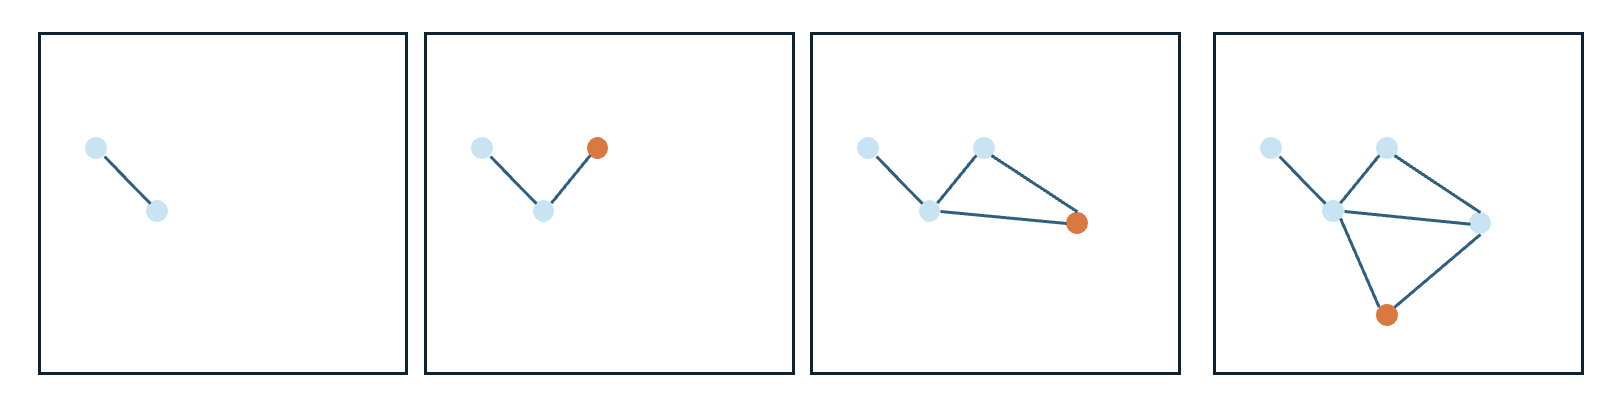
\includegraphics[scale=0.55]{../img/theory/preferential_attachement.png}
    \caption{Illustration of the Barabási-Albert model. Each step adds one node and connects it to other nodes with a probability proportional to their degree. In the figure, we can see that a new node tends to connect to nodes with an already high degree.}
    \label{fig:barabasi_albert}
\end{figure}

\subsection{Configuration model}
The configuration model starts with a prescribed degree sequence ${k_i}$ and tries to find graphs compatible with such that degree sequence. The simplest approach is to start with a desired number of vertices $N$ and assign to each node a number of half-edges that corresponds to its prescribed degree. These half-edges can be connected together to form full edges. One way to do that is to connect them uniformly randomly. That gives a random network model, which yields graphs with a degree sequence precisely corresponding to the prescribed one.

However, this version of the configuration model cannot avoid self-loops (edges going from some node to itself). Therefore, graphs generated by this model can usually hardly be compared with real-world networks. An approach avoiding this issue is called link stub reconnection. It starts with a real-world network without self-loops and reconnects its edges in such a manner that the degree sequence is preserved. However, this method was shown to explore the space of all allowed graphs non-uniformly, staying near the original graph. This can be overcome by introducing an acceptance-probability \cite{Coolen2009}, but that makes the whole problem more computationally demanding.

\begin{figure}[!ht]
    \centering
    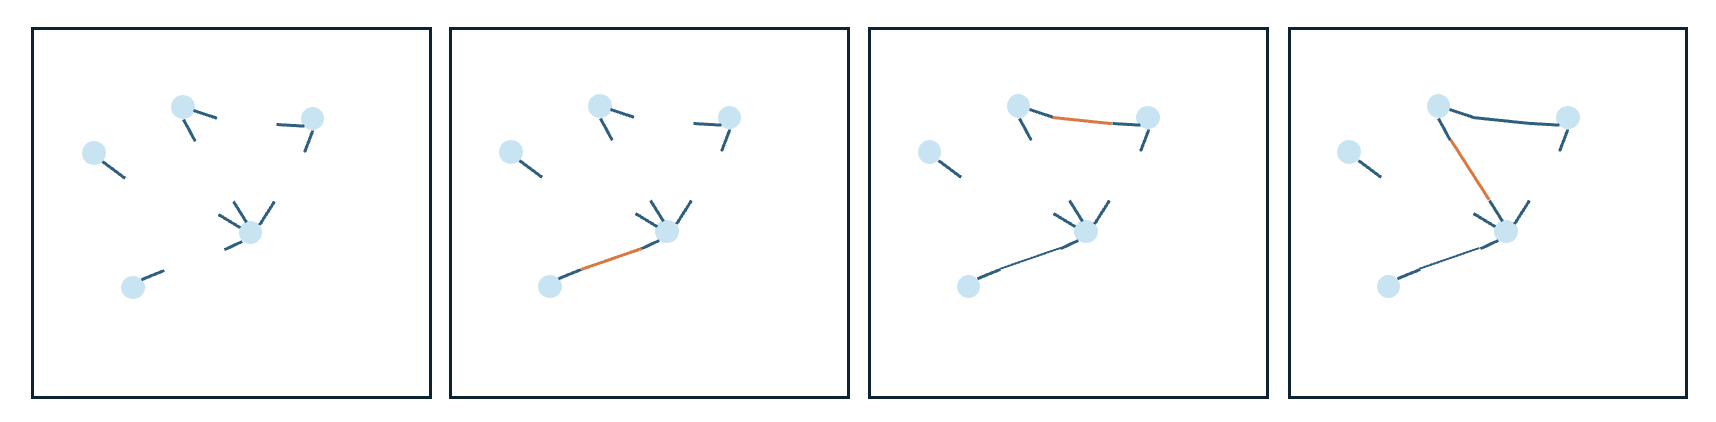
\includegraphics[scale=0.5]{../img/theory/configuration_model.png}
    \caption{Illustration of the configuration model. Each node possesses the so-called half-stubs or half-edges. The number of half-stubs corresponds to the desired degree. Then these half stubs are connected uniformly randomly to form full edges.}
    \label{fig:barabasi_albert}
\end{figure}

\subsection{Maximum-entropy ensembles of graphs}
\label{sec_max_ent_ensembles}
Random network models can not only produce a single realization, but a whole ensemble of graphs. Let us denote $\mathcal{G}$ all possible graphs (where we usually fix the number of nodes, we omit the notation here). Then a random network model essentially assigns a probability $P(G)$ to each graph $G \in \mathcal{G}$, s.t. $\sum_{G \in \mathcal{G}}P(G) = 1$. Let us recall the configuration model. This model was producing an ensemble of graphs with a fixed degree sequence. However, we also encountered several limitations. Essentially, the configuration model creates a microcanonical ensemble, constraint is forced in each realization. 

We can take another approach and only demand our constraints to be valid on average over the whole ensemble. To define a model, we need to assign probabilities to each graph possible. But from statistical physics, we know how to find the least biased probability distributions given constraints, using the maximum-entropy principle. This approach was used similarly for networks by Park and Newman \cite{Park2004}, and we will briefly introduce it here. Similar results were obtained even earlier and the whole mathematical framework is commonly called \textbf{Exponential Random Graphs} (ERG).

The most unbiased choice of probability distribution $P(G)$ over graphs $G \in \mathcal{G}$ is coming from maximizing the Shannon entropy defined as

\begin{equation}
    S = -\sum_{G \in \mathcal{G}}P(G) \ln P(G)
\end{equation}
with normalization $\sum_{G \in \mathcal{G}}P(G) = 1$. The canonical ensemble is obtained by imposing soft constraints
\begin{equation}
    \vec{c^*} = \sum_{G \in \mathcal{G}} \vec{c}(G)P(G)
\end{equation}

where $\vec{c^*}$ are the constraints we want to recover in expected value over the ensemble. In constrained maximization, these constraints are coupled with Lagrange multipliers $\vec{\theta}$ and the maximization problem yields, similarly to statistical mechanics

\begin{equation}
    P(G|\vec{\theta}) = \frac{e^{-H(G,\vec{\theta})}}{Z(\vec{\theta})}
\end{equation}

where $H(G,\theta) = \vec{c}(G)\cdot\vec{\theta}$ is the graph Hamiltonian and $Z(\vec{\theta}) = \sum_{G \in \mathcal{G}}e^{-H(G,\theta)}$ is the partition function.

Also similarly to statistical mechanics, we can introduce the free energy $F(\vec{\theta}) = -\ln Z(\vec{\theta})$ and obtain

\begin{equation}
    \mathbb{E}(c_\alpha) = \pder{F(\vec{\theta})}{\theta_\alpha}
\end{equation}

\subsubsection{Undirected case}
Let us consider the following Hamiltonian:
\begin{equation}
    H(G,\vec{\theta}) = \sum_{i<j} \theta_{ij}a_{ij}
\end{equation}

where $a_{ij}$ are the elements of the adjacency matrix of $G$. Then one can compute the partition function analytically

\begin{equation}
    Z(\vec{\theta}) = \sum_{\{a_{ij}\}} e^{-\sum_{i<j} \theta_{ij}a_{ij}} =  \sum_{\{a_{ij}\}}\prod_{i<j}e^{-\theta_{ij}a_{ij}} = \prod_{i<j} \sum_{\{a_{ij} = 0,1\}}e^{-\theta_{ij}a_{ij}} = \prod_{i<j}(1 + e^{-\theta_{ij}})
\end{equation}
and therefore the free energy is
\begin{equation}
    F(\vec{\theta}) = -\sum_{i<j}\ln(1 + e^{-\theta_{ij}})
\end{equation}
Let us note, that this is a model with independent edges. That is because the probability of the whole graph factorizes into probabilities depending only on single edges:
\begin{equation}
    P(G|\vec{\theta}) = \frac{e^{-\sum_{i<j} \theta_{ij}a_{ij}}}{Z(\vec{\theta})} = \frac{\prod_{i<j}e^{-\theta_{ij}a_{ij}}}{{Z(\vec{\theta})}}
\end{equation}

Then the probability, that node $i$ and $j$ are connected is
\begin{equation}
    p_{ij} = \mathbb{E}(a_{ij}) = \pder{F(\vec{\theta})}{\theta_{ij}} = \frac{1}{1 + e^{\theta_{ij}}}
\end{equation}
Remarkably, this result reminds us of the Fermi-Dirac statistics. That is not a coincidence, since each edge is either present or not present, which corresponds to a state which can be occupied by at most one particle, like in the fermionic case.

Now let us consider two cases:
\begin{itemize}
    \item Setting $\theta_{ij} = \theta$: Then the Hamiltonian is $H(G,\theta) = \sum_{i < j}\theta a_{ij} = \theta L_u(G)$, where $L_u(G)$ is the total number of links in $G$. Therefore, this Hamiltonian corresponds to only constraining the total number of links. Then $p_{ij} = \frac{1}{1 + e^{-\theta}}$, i.e. the same for all nodes and we recover the Erdős-Rényi model.
    \item Setting $\theta_{ij} = \theta_i + \theta_j$: Then 
    \begin{equation}
        H(G,\theta) = \sum_{i < j}(\theta_i + \theta_j) a_{ij} = \sum_{i\neq j}\theta_i a_{ij} = \sum_{i\neq j}\theta_i k_i(G)
    \end{equation}where $k_i(G)$ is the degree of i-th node of the graph $G$. This corresponds to constraining the degrees of nodes, therefore this is the canonical version of the configuration model. The link probabilities are
    \begin{equation}
        p_{ij} = \frac{1}{1 + e^{\theta_i + \theta_j}} = \frac{1}{1 + e^{\theta_i}e^{\theta_j}} = \frac{x_i x_j}{1 + x_i x_j}
    \end{equation}
    where we used the reparametrization $x_i = e^{-\theta_i}$. This model is usually called the Park-Newman model or the \textit{binary-configuration model} (BCM).
\end{itemize}

\subsubsection{Directed case}
In the directed case, the adjacency matrix does not have to be symmetric, and therefore we can assign a Lagrange multiplier to each of its entries (we exclude the diagonal entries - self-loops). Let us therefore write the Hamiltonian
\begin{equation}
    H(G,\vec{\theta}) = \sum_{i\neq j} \theta_{ij}a_{ij}
\end{equation}
Analogically, we have
\begin{align}
    Z(\vec{\theta}) &= \prod_{i\neq j}(1 + e^{-\theta_{ij}}) \\
    F(\vec{\theta}) &= -\sum_{i\neq j}\ln(1 + e^{-\theta_{ij}}) \\
    p_{ij} &= \mathbb{E}(a_{ij}) = \pder{F(\vec{\theta})}{\theta_{ij}} = \frac{1}{1 + e^{\theta_{ij}}}
\end{align}

Now, let us show the important case, where
\begin{equation}
    H(G,\vec{\alpha},\vec{\beta}) = \sum_{i\neq j}(\alpha_i + \beta_j)a_{ij} = \sum_i(\alpha_i k_i^{out}(G) + \beta_i k_i^{in}(G))
\end{equation}
This amounts to constraining both the out-degree and in-degree sequence. Then the edge probabilities are
\begin{equation}
    p_{ij} = \frac{1}{1 + e^{\alpha_i + \beta_j}} = \frac{x_i y_j}{1 + x_i y_j}
    \label{eq_DBCM}
\end{equation}
where we reparametrized $x_i \equiv e^{-\alpha_i}$, $y_j \equiv e^{-\beta_j}$. A model where each node $i$ is assigned values $x_i$, $y_i$ and edges are drawn with probability \ref{eq_DBCM} is called \textit{Directed Binary configuration model} (DBCM).

\subsubsection{Maximum likelihood estimation in maximum-entropy models}
Let us recall the maximum likelihood estimation from statistics. Let us have a sample $(X_1, \dots X_n)$ from a given distribution $f(x, \vec{\theta})$ with parameters $\vec{\theta}$ from some set $\Theta$. Then the likelihood of a realization $(x_1, \dots, x_n)$ as a function of parameters $\vec{\theta}$ is
\begin{equation}
    L(\vec{\theta}) = \prod_{i=1}^n f(x_i, \vec{\theta})
\end{equation}
The maximum-likelihood estimation prescribes to find such parameters $\vec{\theta}^{*}$ of the probability distribution, which maximize the likelihood of generating the given realization, i.e.
\begin{equation}
    \vec{\theta}^{*} = \arg\max_{\vec{\theta} \in \Theta} L(\vec{\theta})
\end{equation}
A common practice is not to maximize $L(\vec{\theta})$, but rather its logarithm (log-likelihood) $\lambda(\vec{\theta}) = \ln L(\vec{\theta})$.

Now in case of graphs, let us assume we have one real-world network $G^*$. Then the likelihood of producing such network with some stochastic network model is 
\begin{equation}
    \lambda(\vec{\theta}) = \ln P(G^*|\vec{\theta})
\end{equation}
where $P(G|\vec{\theta})$ is the graph probability distribution of our model with the parameters $\vec{\theta}$. Then we need to find such parameters which maximize this log-likelihood, therefore
\begin{equation}
    \nabla \lambda(\vec{\theta}) = \left[\pder{\lambda(\vec{\theta})}{\vec{\theta}} \right]_{\vec{\theta} = \hat{\vec{\theta}}} = 0
\end{equation}

Now let us consider the maximum-entropy ensemble, where 

\begin{equation*}
    P(G|\vec{\theta}) = \frac{e^{-H(G,\vec{\theta})}}{Z(\vec{\theta})}
\end{equation*}

Then the log-likelihood for a given graph $G^*$ is
\begin{equation*}
% todo
\lambda(\vec{\theta}) \equiv \ln P(G^*|\vec{\theta}) = \ln\frac{e^{-H(G^*,\vec{\theta})}}{Z(\vec{\theta})} = \ln e^{-H(G^*,\vec{\theta})} - \ln Z(\vec{\theta}) = -H(G^*,\vec{\theta}) - \ln Z(\vec{\theta})
\end{equation*}

The partial derivatives with respect to the parameters are (given $H(G,\theta) = \vec{c}(G)\cdot\vec{\theta}$)

\begin{equation*}
\frac{\partial \lambda(\vec{\theta})}{\partial \theta_i} = -c_i (G^*) + \frac{1}{Z(\vec{\theta})} \sum_{G}{c_i (G) e^{-H(G,\vec{\theta})}}
\end{equation*}

Setting equal to zero, we get
\begin{equation*}
    c_i (G^{*}) = \frac{1}{Z(\vec{\theta}^{*})} \sum_{G}{c_i (G) e^{-H(G,\vec{\theta}^{*})}} = \langle c_i \rangle ^*
\end{equation*}
where $\langle c_i \rangle ^*$ is the expected value of $c_i$ evaluated using the parameters $\vec{\theta}^{*}$.

Therefore, if we choose some constraints in the maximum-entropy model, we can then find the corresponding model parameters (Lagrange multipliers) by setting them in such a way that they reproduce (on ensemble average) the quantities we constrained, and this fit is then the one we would as well obtain using the maximum-likelihood estimation. That is a quite remarkable result. 

Thus, the Exponential Random graphs (ERG) give us a general recipe, how to find models reproducing some properties following the maximum-likelihood principle: we just need to include those properties in the Hamiltonian and find the corresponding model to such Hamiltonian.
 
\subsection{The Scale-invariant model (SIM)}
Let us recall renormalization in physics. Consider a system described by some function $Z$ (Hamiltonian, partition function etc.) of states $s_i$ and coupling constants $J_i$. Assume a blocking transformation, which aggregate several states to a new ``block'' state. Therefore, we obtained a smaller state of block-states $\Tilde{s}_i$. Then, if we can find express the system function $Z$ as a function of the new states $\Tilde{s}_i$ and some new coupling constants $\Tilde{J}_i$, we call our model renormalizable. The process of describing the system on a higher scale is called \textbf{coarse-graining}.

Here we want to answer the following question: can we find a random graph model, which remains consistent at different scales, different coarse-graining levels? That means if we choose a different scale, is our system still described by the same model, only with possibly renormalized parameters?

To answer that question, we first need to define, how the coarse-graining would be performed. Garuccio, Lalli and Garlaschelli \cite{Garuccio2023} came up with a model which stays invariant for any desired partition of nodes into block-nodes. Here, we will briefly introduce this model.

\subsubsection{Coarse-graining procedure}
Let us have an undirected graph with $N_0$ nodes. Let us then choose any partitioning of these nodes in $N_1$ non-overlapping groups, each group can be called a block-node. Then, if there exists any connection between nodes from two different groups, we connect these groups as well, otherwise not. This process is visualized on figure \ref*{fig:coarse_graining}.

\begin{figure}[!ht]
    \centering
    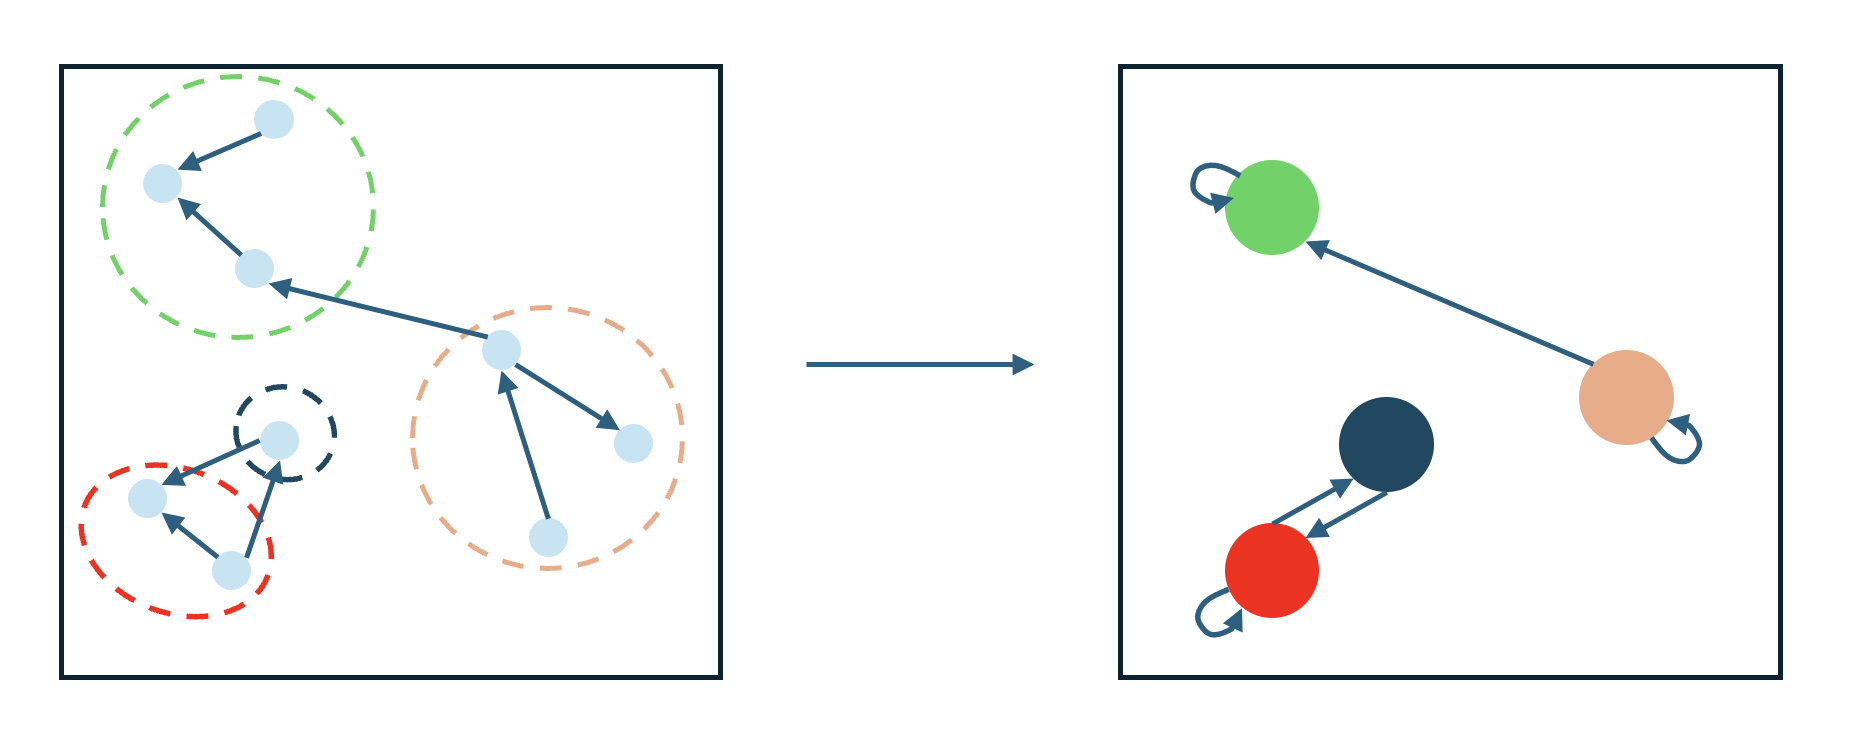
\includegraphics[scale=0.45]{../img/theory/coarse_graining.png}
        \caption{Illustration of one coarse-graining step in the Scale-invariant model. We can form groups of nodes in an arbitrary way. Then groups are connected only if there is any connection between nodes form those groups. If there is a connection between nodes in the same group, self-loop is formed. If there are links in both directions between nodes from two groups, a reciprocated link is formed.}
        \label{fig:coarse_graining}
    \end{figure}

Let us have the adjacency matrix $\mathbb{A}^{(0)}$ of the initial graph with $N_0$ nodes. We denote its elements as $a_{i_0,j_0}^{(0)}$. If there is a link between $i_0$ and $j_0$, then $a_{i_0,j_0}^{(0)} = 1$, otherwise $a_{i_0,j_0}^{(0)} = 0$. Now, if we make the partitioning in $N_1$ groups, the adjacency matrix $\mathbb{A}^{(1)}$ of the new coarse-grained graph will be 
\begin{equation}
    a_{i_1,j_1}^{(1)} = 1 - \prod_{i_0 \in i_1}\prod_{j_0 \in j_1} (1 - a_{i_0,j_0}^{(0)})
\label{eq_coarse_grain}
\end{equation}
where the expression $i_0 \in i_1$ means, that node $i_0$ is contained in the block-node $i_1$. The expression \ref{eq_coarse_grain} corresponds to the requirement, that we do not connect two groups only if there is no connection between any two nodes from the two groups.

We can denote the partitioning of nodes as a function, which assigns every node to its corresponding group, that is $i_1 = \Omega_0(i_0)$. But now, for the new coarse-grained graph, we can find another partitioning, $\Omega_1$ and perform another level of coarse-graining. We obtain the corresponding adjacency matrix $\mathbb{A}^{(2)}$ similarly. In the end, we can make a sequence of partitionings, $\{\Omega_l\}_{l\geq0}$ and find the corresponding sequence of adjacency matrices $\{\mathbb{A}^{(l)}\}_{l\geq0}$. 

Let us make an important remark. The model aims to allow for arbitrary partitioning, therefore it does not rely on any geometrical embedding. That explains the name of the original paper ``Scale-invariance without geometry''. This is also a difference with other proposed renormalization schemes, both in physics, or in network science, which rely heavily on geometry.

\subsubsection{Scale-invariance}
Now we know how to coarse-grain any graph. With that, we would like to find a random graph model, which can generate graphs in a scale-invariant fashion. We explain, what we mean by that, in the following paragraphs.

Let us assume, that the graph at the lowest-level, $\mathbb{A}^{(0)}$ comes from some probability distribution $P_0(\mathbb{A}^{(0)}, \Theta_0)$, where $\Theta_0$ are parameters of the model. We demand a normalization $\sum_{\mathbb{A}^{(0)} \in \mathcal{G}_{N_0}}P_0(\mathbb{A}^{(0)}, \Theta_0) = 1$, where $\mathcal{G}_{N_0}$ denotes all binary undirected graphs with $N_0$ nodes. Now let us fix some partitioning sequence $\{\Omega_l\}_{l\geq0}$. Since we have a probability of each graph $\mathbb{A}^{(0)} \in \mathcal{G}_{N_0}$, what is the probability of the graph $\mathbb{A}^{(1)}$ at the next coarse-graining level? It is just a sum of probabilities of all graphs $\mathbb{A}^{(0)}$, which end up being coarse grained to the graph $\mathbb{A}^{(1)}$, i.e. \begin{equation}
    P_1(\mathbb{A}^{(1)}, \Theta_1) = \sum_{\{\mathbb{A}^{(0)}\} \xrightarrow{\Omega_0} \mathbb{A}^{(1)}} P_0(\mathbb{A}^{(0)}, \Theta_0)
\end{equation}
where the sum goes over all graphs $\mathbb{A}^{(0)}$ projected on $\mathbb{A}^{(1)}$ by the partitioning $\Omega_0$. $\Theta_1$ are some new model parameters. Similarly, we find the probability of a graph in the $l$-th coarse-graining level to be
\begin{equation}
    P_l(\mathbb{A}^{(l)}, \Theta_l) = \sum_{\{\mathbb{A}^{(0)}\} \xrightarrow{\Omega_{l-1}\dots\Omega_0} \mathbb{A}^{(l)}} P_0(\mathbb{A}^{(0)}, \Theta_0)
\end{equation}
where $\Omega_{l-1}\dots\Omega_0$ is just a composition of partitions $\Omega_{0}$,\dots,$\Omega_{l-1}$. 

The requirement of a scale-invariant model means, that if we want to generate graphs in the $l$-th level, we can either first generate them at the 0-th level and then deterministically coarse-grain, or we can generate them directly at the $l$-th level using the same model. That means, the same model should be valid for all coarse-graining levels in its form, where only the parameters of the model and its dimensionality would change. That corresponds to renormalization in physics, where, by changing the scale, we obtain the same functional form of the model, but with renormalized parameters.

The scale-invariance requirement can be therefore written for any $l \in \mathbb{N}$ as
\begin{equation}
    P(\mathbb{A}^{(l)}, \Theta_l) = \sum_{\{\mathbb{A}^{(0)}\} \xrightarrow{\Omega_{l-1}\dots\Omega_0} \mathbb{A}^{(l)}} P(\mathbb{A}^{(0)}, \Theta_0)
\end{equation}
where we dropped the dependence of probability distribution on coarse-graining level $l$, and where the new parameters $\Theta_l$ are obtained only from the parameters $\Omega_0$ and the knowledge of partitionings $\Omega_{0}$,\dots,$\Omega_{l-1}$. This also implies, that we can start from any level in general, not only the 0-th. Therefore, the most general scale-invariance expression for any $l,m\in\mathbb{N}$, $l>m$ reads

\begin{equation}
    P(\mathbb{A}^{(l)}, \Theta_l) = \sum_{\{\mathbb{A}^{(m)}\} \xrightarrow{\Omega_{l-1}\dots\Omega_m} \mathbb{A}^{(l)}} P(\mathbb{A}^{(m)}, \Theta_m)
\label{eq_scale_invariance}
\end{equation}

\subsubsection{Specifying the model}
Now, let us add more requirements to the model. First, we assume, that the edges are \textbf{independent}.  This is a usual setting for random graph models, and it is a crucial simplification. Entries of the adjacency matrix are independent Bernoulli random variables. The probability of link between node $i_l$ and $j_l$ being present is $p_{i_l,j_l}(\Theta_l)$ (we explicitly denote the dependence on $\Theta_l$ and implicitly assume dependence on fitnesses $x_{i_l}, x_{j_l}$ ). In that case, the graph probability factorizes as
\begin{equation}
    P(\mathbb{A}^{(l)}, \Theta_l) = \prod_{i_l=1}^{N_l}\prod_{j_l=1}^{i_l} [p_{i_l,j_l}(\Theta_l)]^{a_{i_l,j_l}^{(l)}}[1 - p_{i_l,j_l}(\Theta_l)]^{1 - a_{i_l,j_l}^{(l)}}
\end{equation}

Next, let us specify the model parameters. First, we assume a global constant $z_l$, which is tuning the overall density at the $l$-th coarse-graining level. Next, let us assign a 'fitness' parameter $x_{i_l}$ to each node $i_l$ in the $l$-th coarse-graining level. These fitness parameters quantify the overall tendency of nodes to connect to other nodes. Then, we can also assign parameters to all possible pairs of nodes, we denote them $\{d_{i_l,j_l}\}_{i_l,j_l=1}^{N_l}$. The final assumption is, that the fitness parameters are node-additive upon coarse-grainings, i.e. $x_{i_{l+1}} = \sum_{i_l \in i_{l+1}} x_{i_l}$ for any coarse-graining level $l$.

\subsubsection{Finding the functional form}
The equation \ref{eq_scale_invariance} with the requirements above is a functional equation where the goal is to find the suitable form of graph probability, or, since the links are independent, the link probability. Let us show the derivation in the case where 
dyadic parameters $\{d_{i_l,j_l}\}_{i_l,j_l=1}^{N_l}$ are not present. 

Let us have two consecutive levels of coarse-graining, $l$ and $l+1$. Scale-invariance demands, that the functional form of link probability is the same at all coarse-graining levels and that only the parameters change by some renormalization rule. Let us assume two distinct blocks $i_{l+1}$, $j_{l+1}$ of nodes at the level $l+1$. We defined our coarse-graining in such way, that these blocks are not connected only if there are no links between any two nodes from these blocks. The probability, that the blocks $i_{l+1}$ and $j_{l+1}$ are not connected is $1 - p_{i_{l+1},j_{l+1}}(z_{l+1})$. This probability depends on the overall density factor $z_{l+1}$ as well as on fitnesses $x_{i_{l+1}}$, $x_{j_{l+1}}$ (we do not denote this dependence and leave it implicit from the subscripts). The links are independent and therefore the probability, that there are no connections between nodes of the two blocks, is equal $\prod_{i_l\in i_{l+1}}\prod_{j_l\in j_{l+1}}[1-p_{i_l,j_l}(z_l)]$. Therefore, the scale-invariance requirement reads
\begin{equation}
    1 - p_{i_{l+1},j_{l+1}}(z_{l+1}) = \prod_{i_l\in i_{l+1}}\prod_{j_l\in j_{l+1}}[1-p_{i_l,j_l}(z_l)]
\end{equation}

Taking logarithm, we obtain
\begin{equation}
    \ln [1 - p_{i_{l+1},j_{l+1}}(z_{l+1})] = \sum_{i_l\in i_{l+1}}\sum_{j_l\in j_{l+1}}[1-p_{i_l,j_l}(z_l)]
\end{equation}

This equation should hold for all pairs from the $l+1$-th coarse-graining level and all possible partitions. The only possible solution is such, that $z_{l+1} = z_l \equiv z$ and
\begin{equation}
     \ln [1 - p_{i_{l+1},j_{l+1}}(z)] = -zg(x_{i_{l+1}})g(x_{j_{l+1}})
     \label{eq_ln_expression}
\end{equation}
where
\begin{equation}
    g(x_{i_{l+1}}) = \sum_{i_l\in i_{l+1}}g(x_{i_l})
\end{equation}
The density parameter $z$ needs to be positive, so that the probability is correctly defined. Function $g$ needs to have same sign for all nodes, and we can therefore choose it to be positive. Also, since we required the fitnesses to be node-additive, and therefore the only possible choice of $g(x)$ is $g(x) = kx$ for some constant $k$. We can then redefine $z \leftarrow k^2 z$ and rewrite \ref{eq_ln_expression} as
\begin{equation}
    \ln [1 - p_{i_{l+1},j_{l+1}}(z)] = -zx_{i_{l+1}}x_{j_{l+1}}
\end{equation}
In the end, for two distinct block-nodes $i_l \neq j_l$, we obtain
\begin{equation}
    p_{i_l,j_l}(z) = 1 - e^{-zx_{i_l}x_{j_l}}, \qquad z, x_{i_l}, x_{j_l} > 0
\end{equation}
In the case, where $i_l = j_l$, one needs to be careful to not double-count the same edges. Then, the derivation (see Appendix 1 in \cite{Garuccio2023}) leads to
\begin{equation}
    p_{i_l,j_l} = 1 - e^{-\frac{z}{2}x_{i_l}^2}, \qquad z, x_{i_l} >0
\end{equation}

Therefore, we obtained the functional form of the link probability from the requirement of scale-invariance. Also, we have a renormalization rule for the density parameter $z_l$, that is $z_l = z_{l+1} \equiv z$, i.e. density parameter remains constant. The renormalization rule for fitnesses was imposed in advance, $x_{i_{l+1}} = \sum_{i_l\in i_{l+1}} x_{i_l}$.

One can also take in the account the dyadic (edge-specific) parameters $\{d_{i_l,j_l}\}_{i_l,j_l=1}^{N_l}$. In that case, we obtain the most general form of the Scale-Invariant Model (SIM) present in \cite{Garuccio2023}
\begin{equation}
    p_{i_l,j_l} = 
    \begin{cases}1 - e^{zx_{i_l}x_{j_l}}f(d_{i_l,j_l}) \quad \text{if} \quad i_l \neq j_l \\
    1 - e^{-\frac{z}{2}x_{i_l}^2}f(d_{i_l,i_l}) \quad \text{if} \quad i_l = j_l \\
    \end{cases}
\end{equation}
where $z>0$, $x_{i_l} \geq 0 \, \forall i_l$ and f is an arbitrary positive function. The renormalization rules for the model parameters are then
\begin{align}
    z_{l+1} &\equiv z_l \equiv z \\
    x_{i_{l+1}} &\equiv \sum_{x_{i_l}\in x_{i_{l+1}}} \\
    f(d_{i_{l+1},j_{l+1}}) &\equiv \frac{\sum_{i_l\in i_{l+1}}\sum_{j_l\in j_{l+1}}x_{i_l}x_{j_l}f(d_{i_l,j_l})}{\sum_{i_l\in i_{l+1}}x_{i_l}\sum_{j_l\in j_{l+1}}x_{j_l}}
\end{align}
Let us point out, that the dependence on the dyadic factors can be eliminated by choosing function $f$ to be a constant function.

\subsubsection{Directed case}
Recently, Lalli and Garlaschelli generalized the Scale-Invariant Model for directed networks (Directed Scale-Invariant Model - DSIM) \cite{Lalli2024}. They tackled the problem, how to reproduce the nontrivial patterns in reciprocity of directed links in real-world network. Reciprocity refers to a non-trivial tendency of nodes to form mutual (reciprocated) connections.

We denote four probabilities for edges between nodes $i_l$ and $j_l$:
\begin{itemize}
    \item $\overset\rightarrow{p_{i_l,j_l}}(\Theta_l)$ for a single directed link from $i_l$ to $j_l$ and no reciprocal link from $j_l$ to $i_l$
    \item $\overset\leftarrow{p_{i_l,j_l}}(\Theta_l)$ for a single directed link from $j_l$ to $i_l$ and no reciprocal link from $i_l$ to $j_l$
    \item $\overset\leftrightarrow{p_{i_l,j_l}}(\Theta_l)$ for a reciprocated link between $i_l$ and $j_l$
    \item $\overset{\not\leftrightarrow}{p_{i_l,j_l}}(\Theta_l)$ for no link between $i_l$ and $j_l$
\end{itemize}
Let us also denote $p_{i_l,j_l}(\Theta_l)$ to be the marginal probability of a link from $i_l$ to $j_l$. The simplest case would be, that we could factorize the four probabilities using the marginal probability, i.e. $\overset\rightarrow{p_{i_l,j_l}}(\Theta_l) = p_{i_l,j_l}(\Theta_l)(1 - p_{j_l,i_l}(\Theta_l))$, $\overset\leftarrow{p_{i_l,j_l}}(\Theta_l) = p_{j_l,i_l}(\Theta_l)(1 - p_{i_l,j_l}(\Theta_l)$ etc. The authors, however, do not assume this, to reproduce non-trivial reciprocity patterns. 

Firstly, every directed graph can be projected to an undirected one (undirected link between two nodes is present if there is a directed link between those two nodes in at least one direction). We demand this undirected projection to follow the undirected SIM. The undirected connection probability between nodes $i_l$ and $j_l$ can be written as 
\begin{align}
    q_{i_l,j_l} = \overset\rightarrow{p_{i_l,j_l}} + \overset\leftarrow{p_{i_l,j_l}} + \overset\leftrightarrow{p_{i_l,j_l}} = 
    \begin{cases}
        1 - e^{-\delta x_{i_l}x_{j_l}f(d_{i_l,j_l})}, \qquad &i_l \neq j_l\\
        1 - e^{-\frac{\delta}{2}x_{i_l}^2f(d_{i_l,i_l}) - \eta w_{i_l}}, \qquad &i_l = j_l
    \end{cases}
\end{align}
Here, compared to the original SIM, the parameter $\eta$ was introduced together with a new node-dependent fitness $w_{i_l}$. This fitness controls separately the tendency of a node to form self-loops, while $\eta$ controls it globally. Similarly to fitnesses $x_{i_l}$, also $w_{i_l}$ is node-additive under coarse-graining. 

Another marginal probability to consider is the overall probability $p_{i_l,j_l}$ to form a directed link from node $i_l$ to $j_l$, regardless of the presence of a link in the opposite direction. By demanding scale-invariance, one can get the expression
\begin{align}
    p_{i_l,j_l} = \begin{cases}
        1 - e^{-\epsilon y_{i_l}z_{j_l}f(d_{i_l,j_l})}, \qquad &i_l \neq j_l\\
        1 - e^{-\frac{\delta}{2}x_{i_l}^2f(d_{i_l,i_l}) - \eta w_{i_l}}, \qquad &i_l = j_l
    \end{cases}
\end{align}
where $\epsilon$ determines the overall density of directed links. Also, two sets of fitness variables were introduced, $\{y_{i_l}\}_{i_l=1}^{N_l}$ and $\{z_{i_l}\}_{i_l=1}^{N_l}$. These are the tendencies of nodes to form out-going and in-going links respectively. They are also node-additive, similarly to SIM. $\epsilon$ remains unchanged under coarse-graining, while $f(d_{i_l,j_l})$ follows the renormalization rule
\begin{equation}
    f(d_{i_{l+1},j_{l+1}}) \equiv \frac{\sum_{i_l\in i_{l+1}}\sum_{j_l\in j_{l+1}}y_{i_l}z_{j_l}f(d_{i_l,j_l})}{\sum_{i_l\in i_{l+1}}y_{i_l}\sum_{j_l\in j_{l+1}}z_{j_l}}
\end{equation}

Since we know that $q_{i_l,j_l} = \overset\rightarrow{p_{i_l,j_l}} + \overset\leftarrow{p_{i_l,j_l}} + \overset\leftrightarrow{p_{i_l,j_l}}$ and $p_{i_l,j_l} = \overset\rightarrow{p_{i_l,j_l}} + \overset\leftrightarrow{p_{i_l,j_l}}$, we can now find all the expressions for $\overset\rightarrow{p_{i_l,j_l}}$, $\overset\leftarrow{p_{i_l,j_l}}$, $\overset\leftrightarrow{p_{i_l,j_l}}$ and $\overset{\not\leftrightarrow}{p_{i_l,j_l}}$. Than one can study, how the local reciprocities $r_{i_l,j_l} = \text{Prob}(i_l \rightarrow j_l|j_l \rightarrow i_l)$, as well as the overall reciprocity $\langle r\rangle$ (fraction of expected value of reciprocated links to expected value of all links) behave. For that, we encourage the reader to find details in \cite{Lalli2024}. 

\section{Network reconstruction problem}
In this section, we will introduce the network reconstruction problem, mainly following the review by Squartini et al. \cite{Squartini2018}
In the network science, the focus was initially on determining the properties of real-world network. Several observations were made:
\begin{itemize}
    \item Power-law degrees: Real-world networks usually have node degrees, which are power-law distributed, there are few hubs with many connections and most of the nodes with little connections.
    \item Small-world effect: Nodes are usually close to each other. That means that if we have two nodes and find the shortest path along edges between them, this path is typically short.
    \item Large clustering: nodes usually form densely connected groups, which are then less connected with each other.
    \item Assortativity: Average nearest neighbor degree is either positively or negatively correlated with the node degree.
\end{itemize}

Based on these properties, scientists were trying to find models which could reproduce them. We saw some of these models in the previous section. In case of many networks, for example financial ones, another problem can arise. The information about networks in question is often not complete. In case of financial networks, the detailed data are usually not disclosed and only some limited information is available. We can think of a network of banks, which lend to each other. Banks do not disclose every single liability, they only have to announce their overall exposure. On the other hand, knowledge of such a network or its properties is of a high importance, for example to determine the level of risk in case of a crisis. Therefore, it is important to find methods which can reproduce networks well enough even with the limited knowledge. 

Let us now specify the problem setting. We are interested in reconstructing a weighted directed network defined by its $N \times N$ weight-matrix $\hat{W}$. Its entries $\hat{w}_{ij}$ are non-negative real-numbers and the corresponding adjacency matrix can be found by setting $\hat{a}_{ij} = 1 \iff w_{ij} > 0$ and $\hat{a}_{ij} = 0 \iff w_{ij} = 0$
The weights are not directly observable, the only information we have are the node strengths: 
\begin{equation}
    \hat{s}_i^{out} = \sum_{j=1}^N \hat{w}_{ij} \qquad \hat{s}_i^{in} = \sum_{j=1}^N \hat{w}_{ji}
    \label{eq_strength_constraint}
\end{equation}
Sometimes, degrees $\hat{k}_i^{in}$, $\hat{k}_i^{out}$ could be also available. The typical example of such network is the already mentioned matrix of interbank exposures, also called \textit{liability matrix}. 
Then the general goal is to find two matrices, $P$ and $W$, whose entries correspond to probabilities $p_{ij}$ that nodes $i$ and $j$ are connected and $w_{ij}$ the estimates of the edge weight, if they are connected. The available data are of the order $O(N)$, but we need to find $2N^2$, numbers, therefore the problem is under-determined, and we need a statistical approach. In what follows, we will explore few important examples of reconstruction methods. Interested reader can find more in \cite{Squartini2018}.

\subsection{The MaxEnt algorithm}
The MaxEnt algorithm prescribes to maximize the following functional
\begin{equation}
    S = -\sum_{i,j=1}^N w_{ij}\ln w_{ij}
    \label{eq_max_ent_entropy}
\end{equation}
That is an entropy where the probability distribution is given by weights $w_{ij}$. Maximizing \ref{eq_max_ent_entropy} given the constraints \ref{eq_strength_constraint}, we obtain
\begin{equation}
    w_{ij}^{ME} = \frac{\hat{s}_i^{out}\hat{s}_j^{in}}{\hat{W}} \qquad \forall i, j
\end{equation}
where $\hat{W} = \sum_{i=1}^N \hat{s}_i^{out} = \sum_{i=1}^N \hat{s}_i^{in}$. This model is also known from economics as \textit{gravity model}.

We can see, that unless some strength is equal zero, all the weights have non-zero values, therefore we get the corresponding adjacency matrix has all entries equal to 1 and the obtained network is fully connected. That is the biggest disadvantage of this approach - we can not reconstruct any topological properties of the network of interest. Real-world networks are usually very sparse, and therefore a fully-connected network can not serve as a good approximation. Also, the MaxEnt algorithm is deterministic - it returns only one possible configuration. However, we ideally want a more robust model, which would generate a whole ensemble.

\subsection{Directed Weighted Configuration Model}
Let us recall, that in the section \ref{sec_max_ent_ensembles}, we found the so called Directed Binary Configuration Model using the ERG approach with the Hamiltonian $H(G) = \sum_{i=1}^N (\alpha_ik_i^{out}(G) + \beta_i k_i^{in}(G))$. This Hamiltonian corresponds to constraining the node degrees. In the Directed Weighted Configuration Model, we constrain the strengths instead:
\begin{equation}
    H(\textbf{W}) = \sum_{i=1}^N (\gamma_i s_i^{out}(\textbf{W}) + \delta_i s_i^{in}(\textbf{W}))
\end{equation}
This Hamiltonian also allows the resulting graph probability distribution to factorize in simple pairwise distributions $q_{ij}^{DWCM}(w)$:
\begin{equation}
    P(\textbf{W}) = \prod_{i=1}^N \prod_{j(\neq i)=1}^N q_{ij}^{DWCM}(w)
    \label{eq_prob_factorization}
\end{equation}
Computing the probability distribution $q_{ij}^{DWCM}(w)$ in the case of non-negative integer values of $w$, one finds the geometric distribution
\begin{equation}
    q_{ij}^{DWCM}(w) = (y_i^{out}y_j^{in})^w(1-y_i^{out}y_j^{in}) 
\end{equation}
using the reparametrization $y_i^{out} = e^{-\gamma_i}$ and $y_i^{in} = e^{-\delta_i}$. Since the distribution is geometric, one can easily find the expected value:
\begin{equation}
    \langle w_{ij}^{DWCM} \rangle = \frac{y_i^{out}y_j^{in}}{1 - y_i^{out}y_j^{in}}
\end{equation}
The probability that nodes $i$ and $j$ are connected is given by the probability that $w > 0$, which is
\begin{equation}
    p_{ij}^{DWCM} = \sum_{w=1}^\infty  q_{ij}^{DWCM}(w) = y_i^{out}y_j^{in}
\end{equation}
How are the corresponding reparametrized Lagrange multipliers found? Since the model comes from the ERG framework, we know from section \ref{sec_max_ent_ensembles} that the maximum-likelihood estimation corresponds to setting the ensemble averages equal to the empirical properties we included in the Hamiltonian, i.e. we want to solve the equation
\begin{align}
     \hat{s}_i^{out} &= \langle s_i^{out} \rangle \equiv \sum_{j(\neq i)} \langle w_{ij}^{DWCM} \rangle \qquad \forall i \\
    \hat{s}_i^{in} &= \langle s_i^{in} \rangle \equiv \sum_{j(\neq i)} \langle w_{ji}^{DWCM} \rangle \qquad \forall i
\end{align}
This model, however, also usually generates very dense networks, since the observed strengths are usually large and the corresponding connection probabilities are close to 1. Therefore, to reproduce network topology as well, we need some improvements. 

\subsection{Directed Enhanced Configuration Model (DECM)}
First attempt can be to take degree sequences directly into account. That can be achieved by the Hamiltonian
\begin{equation}
    H(\textbf{W}) = \sum_{i=1}^N (\alpha_i k_i^{out}(G) + \beta_i k_i^{in}(G) + \gamma_i s_i^{out}(\textbf{W}) + \delta_i s_i^{in}(\textbf{W}))
\end{equation}
The probability distribution factorizes similarly to \ref{eq_prob_factorization}, but this time with the link-weight probability
\begin{align}
    q_ij^{DECM}(w) = \begin{cases}
        1 - p_{ij}^{DECM} \qquad &\text{if } w=0 \\
        p_{ij}^{DECM}(y_i^{out}y_j^{in})^{w-1}(1-y_i^{out}y_j^{in}) &\text{if } w>0
    \end{cases}
\end{align}
and link probability
\begin{equation}
    p_{ij}^{DECM} = \frac{x_i^{out}x_j^{in}y_i^{out}y_j^{in}}{1 + x_i^{out}x_j^{in}y_i^{out}y_j^{in} - y_i^{out}y_j^{in}}
    \label{eq_DECM_weight_prob}
\end{equation}
where $x_i^{out} = e^{-\alpha_i}$, $x_i^{in} = e^{-\beta_i}$, $y_i^{out} = e^{-\gamma_i}$, $y_i^{in} = e^{-\delta_i}$. Since the weight distribution is geometric as well, we can easily evaluate the expected weight
\begin{equation}
    \langle w_{ij}^{DECM} \rangle = \frac{p_{ij}^{DECM}}{1 - y_i^{out}y_j^{in}}
    \label{eq_DECM_average_weight}
\end{equation}
and we can find the corresponding Lagrange multipliers in the similar manner, i.e. setting the ensemble averages of degrees and strengths to the empirically observed values.

The disadvantage of this model is, that we need to know all the degrees of the empirical network, which is, however, usually not the case.

\subsection{Fitness-induced DECM}
One way to deal with the problem of missing degree information, is to use the so-called \textit{fitness ansatz}. It assumes that each node carries an intrinsic value, \textit{fitness}, which regulates its connectivity to other nodes and which is directly connected to the Lagrange multipliers coupled to degrees in the ERG framework. As mentioned in \cite{Squartini2018}, strengths usually serve well as fitnesses, meaning that one could express $x_i^{out} = f(\hat{s}_i^{out})$ and $x_i^{in} = f(\hat{s}_i^{in})$ for some function $f$. In the case of financial systems, it has been shown that the form $x_i^{out} = \sqrt{z}\hat{s}_i^{out}$, $x_i^{in} = \sqrt{z}\hat{s}_i^{in}$ works well enough. 

One could then propose a two-step model:
\begin{enumerate}
    \item First estimate the degrees in the network using the $DBCM$ model and use the fitness ansatz, leading to a link probability
    \begin{equation}
        p_{ij}^{f-DBCM} = \frac{z\hat{s}_i^{out} \hat{s}_j^{in}}{1 + z\hat{s}_i^{out} \hat{s}_j^{in}}
    \end{equation}
    where the parameter $z$ can be found using the knowledge of the total number of links $\hat{L}$ equating it to the ensemble average of the total number of links, or we could use a knowledge of connectivity of some subset of nodes. 
    \item Using the link-probabilities from the first step in the DECM model, i.e. in equations \ref{eq_DECM_weight_prob} and \ref{eq_DECM_average_weight}, we replace $p_{ij}^{DECM}$ with $p_{ij}^{f-DBCM}$
\end{enumerate}
The DECM model can be very accurate, but also very computationally-demanding. 
\subsection{Degree-corrected Gravity Model}
\label{sec_DCGM}
A simpler alternative to the DECM model is the so-called Degree-corrected Gravity Model. Here, we also use the connection-probabilities using the DBCM and the fitness ansatz, but we assign weights using the MaxEnt recipe:
\begin{align}
    w_{ij}^{dcGM} = \begin{cases}
        0 \qquad &\text{with probability } 1 - p_{ij}^{f-DBCM}\\
        \frac{w_{ij}^{ME}}{p_{ij}^{f-DBCM}} &\text{with probability } p_{ij}^{f-DBCM}
    \end{cases}
\end{align}
Using this method, we get that on average the weight in this model correspond to those from the MaxEnt recipe
\begin{equation}
    \langle w_{ij}^{dcGM} \rangle = 0\cdot (1 - p_{ij}^{f-DBCM}) + \frac{w_{ij}^{ME}}{p_{ij}^{f-DBCM}}\cdot p_{ij}^{f-DBCM} = w_{ij}^{ME}
\end{equation} meaning, that we reproduce the node strengths well, but we can also tune the parameter $z$ in $p_{ij}^{f-DBCM}$ to reproduce the network density correctly.

\subsection{Comparison on real-world data}
In 2018, a big comparison of several network reconstruction models was conducted by authors from many different central banks across the world \cite{Anand2018}. The authors have access to datasets of interbank loan networks, which is not the case for most of the researchers. The study was conducted over 25 different financial network datasets.

Seven reconstruction methods were tested, out of which four were deterministic and three generated ensembles. We will not dive deep into the comparison, we will just mention, that the Degree-corrected Gravity Model was found to be the ``clear winner across all measures of interest'' among the probabilistic methods. 
\chapter{Experiments}
Now let us present a new approach, namely using the Scale-Invariant Model for network reconstruction. Where can this be useful? We saw, that the Scale-Invariant model describes networks consistently at different scales. Let us imagine a following situation: we want to study systemic risk in an interbank loan network. We know information about banks in the Czech Republic, therefore each of them can form a node in our network model, however, we have no information about banks in China, only their total exposure to Czech banks and vice versa. Therefore, China would only form one node. We clearly have two very different scales present in our network. Ordinary network models might handle this situation inaccurately, however the Scale-invariant model stays consistent even when there are multiple different scales present in the same network.

Let us formulate the problem in terms of interbank loan network. Assume we have $N$ banks labeled $1,\dots N$. We construct a liability matrix in the following way: if bank $i$ a lends money to bank $j$, then the amount lent will be the matrix entry $w_{ij}$. Thus, we obtain a weight-matrix $\hat{W}$ and a corresponding weighted directed graph. We denote the total amount lent by bank $i$ to all other banks (its assets) as $x_i \equiv \sum_{j=1} w_{ij} \equiv hat{s}^{out}$. We also denote the total amount which was lent \textit{to} bank $i$ (its liabilities) as $y_i \equiv \sum_{j=1}^N w_{ji} \equiv \hat{s}^{in}$. These total assets and liabilities are usually the only information disclosed publicly, while the details of the liability matrix are not known. 

\section{Network reconstruction using the original SIM}

Our approach will be similar as in the case of the Degree-corrected Gravity Model \ref{sec_DCGM}, but instead of the link probability from the fitness-induced DBCM model, we will use the Scale-invariant Model. Our approach is therefore as follows:

\begin{enumerate}
    \item We start with the information of the out-strengths $x_i \equiv s_0^{out}$ and in-strengths $y_i \equiv \hat{s}^{in}$ of each node (we call them \textbf{empirical strengths}) and the total number of links $\hat{L}$ (the subscript 0 denotes that it is a property of the original, empirical graph). 
    \item To use the Scale-invariant model, we need to estimate the value of $z$. For that, we demand the ensemble-average of the link-number to be equal to the number of links of the empirical network and find the corresponding $z$. The link probability between node $i$ and $j$ is for given $z$ 
    \begin{equation}
        p_{ij}^{SIM} = 1 - \exp(-z x_i y_j)
        \label{eq_prob_SIM}
    \end{equation}
    and thus we find the value of $z$ by solving the equation
    \begin{equation}
        \langle L \rangle = \mathbb{E}(\sum_{i,j=1}^{N} a_{ij}) = \sum_{i,j=1}^{N} p_{ij} = \sum_{i,j=1}^{N} (1 - \exp(-z x_i y_j)) \overset{!}{=} \hat{L}
        \label{eq:z_fit}
    \end{equation}
    \item We generate an ensemble of $M$ graphs, where $M$ is large enough. Usually, we generate 1000 graphs. Each graph is generated by sampling edges independently using the edge probability \ref{eq_prob_SIM} with corresponding strengths $x_i$, $y_j$ and $z$ from the previous step. When the graph is sampled, we assign weights to its edges in the same way as in the Degree-corrected Gravity Model, i.e.
    \begin{equation}
        w_{ij} = \begin{cases}
            0 \qquad &\text{if } a_{ij} = 0\\
            \frac{x_i y_j}{\tilde{W} p_{ij}^{SIM}} &\text{if } a_{ij} = 1
        \end{cases}    
    \end{equation}
    where $\tilde{W} \equiv \sum_{i=1}^N x_i =  \sum_{i=1}^N y_i$
    \item The generated ensemble is our reconstruction of the empirical network. If we know the empirical network, we can use it to determine the quality of our reconstruction. 
\end{enumerate}

We shall mention an important fact. The Scale-invariant model is proposed in such a way that it stays valid at any level of coarse-graining. However, that is not true for the way we assign weights in the point 3. When we coarse-grain, it is not equivalent to first assign weights to each edge and the sum the corresponding weights together vs. assigning weights at the coarse-grained level using the same formula. We would need to find a scale-invariant model for weighted graphs, which has been only tackled by one master's thesis yet \cite{Verteletskyi}.

\subsection{The dataset}
Our aim is to use this method in the networks of interbank loans. To evaluate the method, we would need to find a dataset with a full interbank loan network. Unfortunately, there is no such dataset freely available. Therefore, we need to find a dataset similar enough. 

For our purposes, we will use the US Airport Network. The dataset contains data for 25 years (1990-2015) of flights between cities in the US\footnote{More information about the dataset can be found at \href{https://ericmjl.github.io/Network-Analysis-Made-Simple/05-casestudies/02-airport/}{https://ericmjl.github.io/Network-Analysis-Made-Simple/05-casestudies/02-airport/}}. If there is a connection between those two cities, the dataset contains the number of passengers taking that connection in a given year. 

Therefore, we can construct a graph, where vertices are airports, edge is present if there is a connection between two different airports and the edge weights are the numbers of passengers on that route. By that, we obtain a directed weighted graph. 

Such a dataset might be similar to the interbank loan network. There is a wide heterogeneity in the size of airports, same as the size of banks. On the other hand, in the airport network, we expect a high reciprocity - if there is a link between A and B with some number of passengers, there is probably a link from B to A with a similar number of passengers. That might not be the case in the interbank networks, as we do not necessarily expect each loan to be reciprocated (actually, we expect the opposite). 

Let us take only the data from the year 2015. We only take those airports which have at least one out-coming and one in-coming connection (non-zero out- and in-strength). In such case, we obtain a network with 1021 vertices and $19\mathpunct{}199$ edges. The number of all possible edges (pairs of nodes) is $1\mathpunct{}042\mathpunct{}441$, therefore our network can be still considered sparse. 

Figure \ref*{fig:deg_strengths} shows the log-log plots of degree and strength distributions. We can see that the out-degree distribution might be fitted by a power-law (straight line in the log-log plot). Gabrielli et al. \cite{Gabrielli2024} study an empirical interbank dataset and find a good fit of the strength distribution using a log-normal distribution. On our plot, however, we can see that although the distribution is decaying fast for high strengths, low strengths do not decay fast enough for the distribution to be log-normal. We could propose to only take vertices with strengths higher than some threshold, but for further purposes we will keep the original data.

\begin{figure}[!ht]
    \centering
    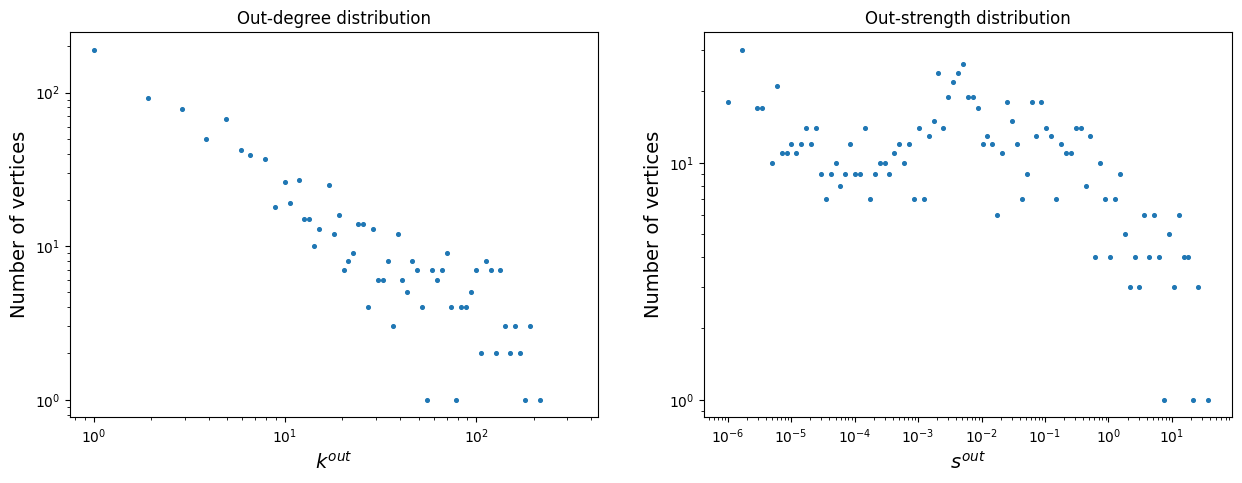
\includegraphics[scale=0.5]{../img/vanilla_SIM/deg_strengths.png}
    \caption{Out-degree and out-strength histograms for the airport network.}
    \label{fig:deg_strengths}
\end{figure}

\subsection{Reconstruction}
Now we can follow the recipe shown above. First, we need to find the value of $z$, that will reproduce the number of links correctly. We solve the equation \ref{eq:z_fit} using bisection method. To avoid numerical problems, we divide all strengths by $10^6$, since the largest strength in our dataset is $44\mathpunct{}337\mathpunct{}603$. By that, we obtained $z \doteq 0.2837$.

Next, we generate an ensemble of 1000 graphs using the Scale-invariant model. The first consistency check is to find the average number of links in our ensemble. That is, for our ensemble, $19\mathpunct{}198.329$, which is close enough to the $19\mathpunct{}199$ edges of the original ensemble.

Next, we can compare properties of the empirical graph and our ensemble. For directed properties (like strengths: out-strengths and in-strengths), we will always show the out-properties, as we did not observe significant difference between the directions.

\subsubsection{Degrees and strengths}
The question of network reconstruction is: can we reproduce the properties of the empirical network by our ensemble on average? This needs to be shown by comparison. Let us first compare these properties node by node. For each node, we can compute the desired property in the empirical graph and also in each graph in the ensemble. Then, for each node, we average its property over the ensemble. 

Figure \ref*{fig:deg_strengths_rec} shows the comparison of empirical degrees and strengths. We can see that strengths are reconstructed very well over the ensemble. Only for nodes, which have low strength in the original ensemble, the reconstruction gets worse, but that is probably due to the limited size of the ensemble. On the other hand, we can see that the degrees are reconstructed on average well only in the high-strength regime. For lower strengths, we see that ensemble averages get below 1, but the degrees in the empirical ensemble are never below one, since there are no isolated nodes.

\begin{figure}[!ht]
    \centering
    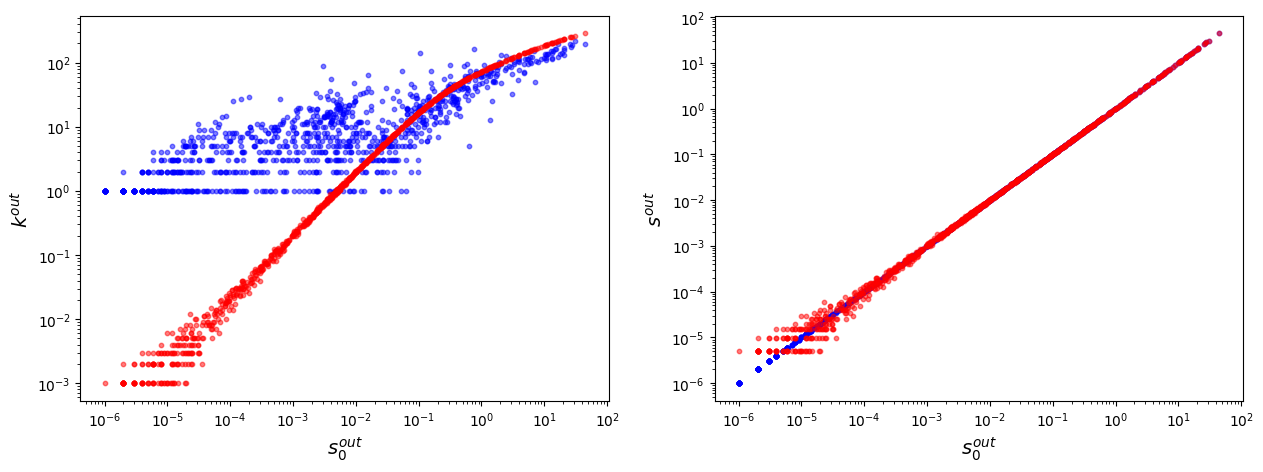
\includegraphics[scale=0.5]{../img/vanilla_SIM/deg_strengths_rec.png}
    \caption{Comparison of out-degrees and out-strengths. Blue points are nodes in the original ensemble, red points are averages of degrees or strengths over the ensemble for each node. Properties are compared against the $s_0^{out}$, the empirical out-strengths (strengths from the empirical ensemble).}
    \label{fig:deg_strengths_rec}
\end{figure}

One can also compare the degree and strength histograms. For each network in the ensemble, we can compute its own degree and strength histogram, and then average them. The result can be found on figure \ref*{fig:deg_strengths_hist_rec}. We can observe two interesting phenomena. First, the model reproduces the degree distribution considerably well, however, it generates certain number of nodes with much higher degree, than what was observed in the empirical graph and underestimates the number of low-degree nodes on the other hand. Second, the strength distributions in the ensemble do not show any nodes with strengths lower than $10^{-3}$, however the strengths in the empirical graph go as low as $10^{-6}$. This can be also probably ascribed to the absence of isolated nodes in the empirical graph. The nodes with low empirical strengths end up being isolated in reconstructed graphs, therefore having zero strength.

\begin{figure}[!ht]
    \centering
    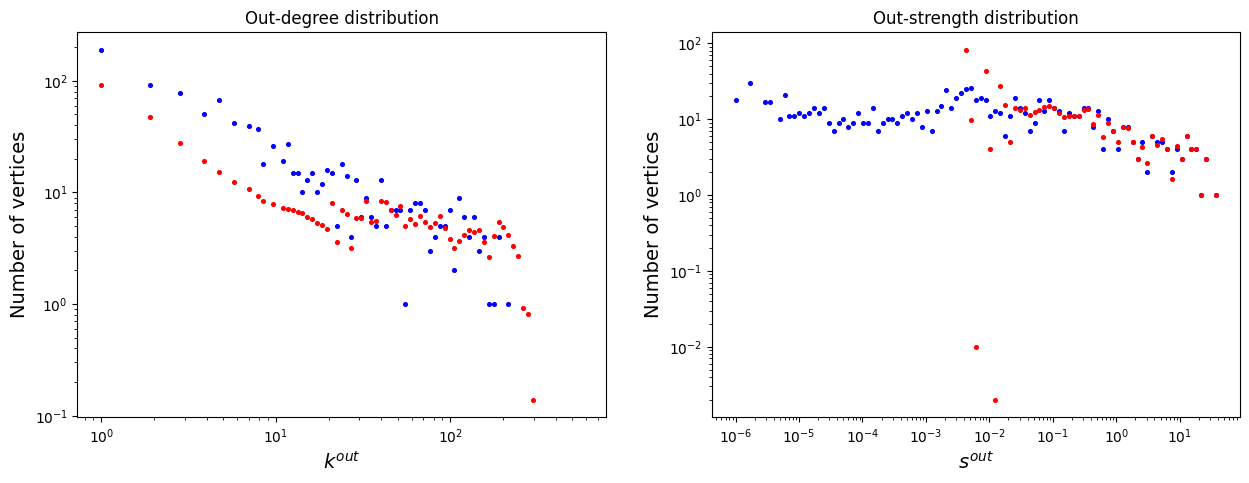
\includegraphics[scale=0.5]{../img/vanilla_SIM/deg_strengths_hist_rec.png}
    \caption{Comparison of degree histograms for the empirical network (blue) and the reconstructed ensemble (red). We can observe that our method produces nodes with higher degrees than what are present in the empirical network. On the other hand, it does not produce nodes with strengths lower than $10^{-3}$.}
    \label{fig:deg_strengths_hist_rec}
\end{figure}

\subsubsection{Average nearest-neighbor degree and local clustering coefficient}
Since we assigned strengths in a way to reconstruct them well on average, we should not be surprised, that they actually were reproduced quite well. The more interesting thing is to study higher order properties like average nearest-neighbor degree or local clustering coefficient. If these can be reproduced well, we have a sign that our reconstruction method works well. 

On figure \ref*{fig:ANND_ANNS}, we can see the comparison of average nearest-neighbor degree (ANND) and average nearest-neighbor strength for each node. We can see that ANND approaches good reconstruction for nodes with high empirical strengths, but for the rest of the nodes, ANND is mostly overestimated. This can be connected with the problem we saw on the histogram \ref*{fig:deg_strengths_hist_rec}, that low degree nodes are underestimated and there are some nodes in the reconstructed ensemble with significantly higher degrees than in the empirical graph.

\begin{figure}[!ht]
    \centering
    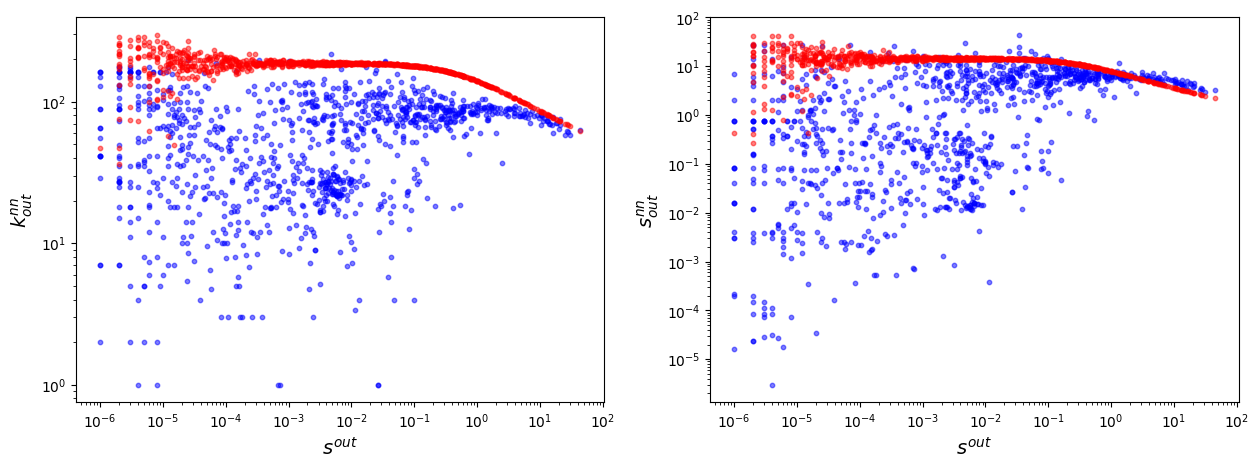
\includegraphics[scale=0.5]{../img/vanilla_SIM/ANND_ANNS.png}
    \caption{Comparison of ANND and ANNS for the empirical graph (blue) and the reconstructed ensemble (red). On the x-axis, there are the empirical strengths.}
    \label{fig:ANND_ANNS}
\end{figure}

Another comparison which is done in the field of network reconstruction, is aggregating nodes with the same degree in groups and for each group computing the average of some property, for example ANND or the local clustering coefficient. We can see such comparison for the ANND on figure \ref*{fig:ANND_k}. Here the overestimation of ANND is even more pronounced. ON the other hand, disassortative tendency (high-degree nodes have on average lower degree neighbors) is reconstructed well.

\begin{figure}[!ht]
    \centering
    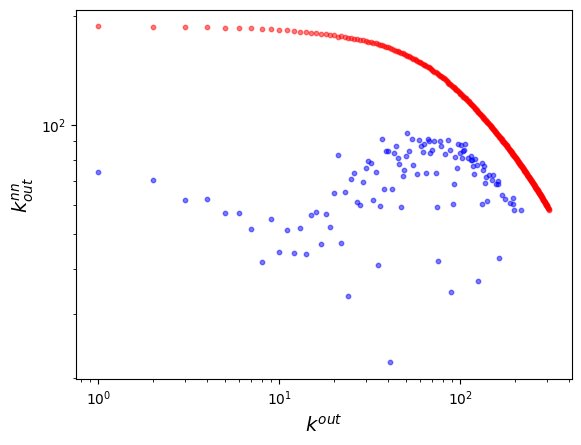
\includegraphics[scale=0.5]{../img/vanilla_SIM/ANND_k.png}
    \caption{Comparison of ANND and ANNS for the empirical graph (blue) and the reconstructed ensemble (red). On the x-axis, there are the empirical strengths.}
    \label{fig:ANND_k}
\end{figure}

We may compare local clustering coefficient as well (see figure \ref*{fig:cl_coeff}). Similarly to ANND, the decreasing tendency of the clustering coefficient is reconstructed well and also the nodes with high empirical-strength show a good correspondence. On the other hand, lower strength nodes have usually higher ensemble-average clustering coefficient than in the empirical graph.

\begin{figure}[!ht]
    \centering
    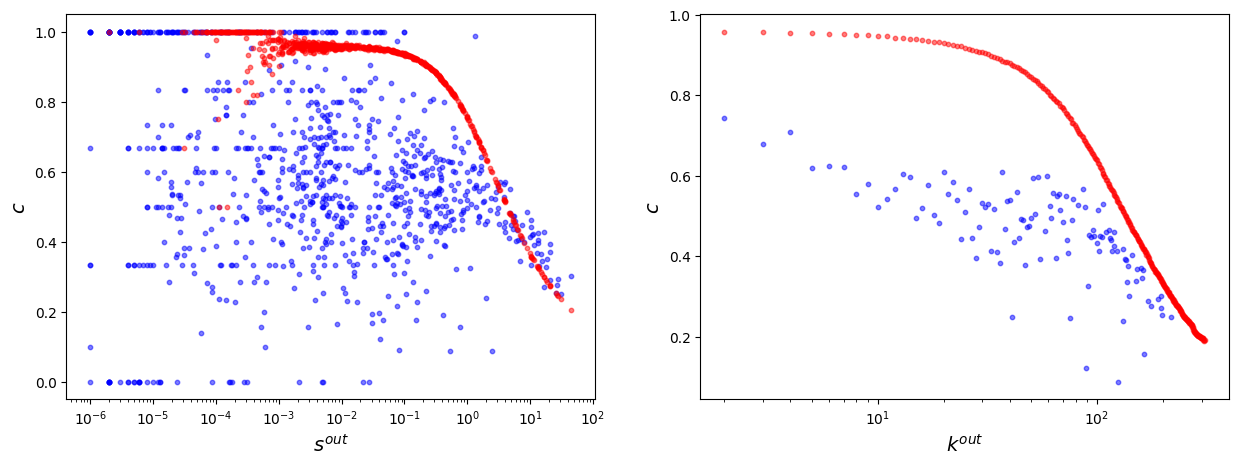
\includegraphics[scale=0.5]{../img/vanilla_SIM/cl_coeff.png}
    \caption{Comparison of the local clustering coefficient for the empirical graph (blue) and the reconstructed ensemble (red). The graph on the left compares each node depending on its empirical strength. The graph on the right shows the aggregated local clustering coefficient for each node degree.}
    \label{fig:cl_coeff}
\end{figure}


\subsubsection{Isolated nodes}
Since we observed, that isolated nodes can pose a problem in the network reconstruction, let us compute, how many of them are there in the reconstructed networks. Let us remind, that the empirical graph has zero isolated nodes, each node has at least one out-going link and one in-going link.

We computed average numbers of out-isolated nodes (nodes with no out-going links) and in-isolated nodes (nodes with no in-going links). Out of 1021 nodes, there were on average 502.745 out-isolated nodes and 503.166 in-isolated nodes. This is remarkably \textbf{bad} result for the financial network reconstruction. 

\section{Degree corrected SIM}
The problem of isolated nodes is actually a crucial one in the financial network analysis. Usually, we want to study dynamical processes, where some signal spreads through the network. For example, the DebtRank model \cite{Bardoscia2015} studies, how the stress spreads in the network when some bank loses a significant portion of its equity. In some cases, the network can dissipate such stress, but also a big bank crisis can occur. If our reconstruction method generates isolated nodes, these do not take part in the stress propagation and our analysis can not be valid. 

We saw that we can not stick to the original model, if we want to avoid too many isolated nodes. Therefore, we want to find such an extension of the scale-invariant model, which imposes some additional constraints while still keeping the scale-invariant properties.

How to extend the SIM in the most ``minimal'' way? We can sample from the original SIM, but then throw away those realizations, which contain isolated nodes. This seems trivial, however generating even one such sample could be very much time-consuming. We thus need to find a more clever sampling strategy.

\subsection{The naive approach}
Let us assume, that every node has out-degree greater or equal than 1, while we do not have requirements on in-degrees (the opposite situation - nonzero in-degrees and no requirements for out-degrees - could be considered analogously). How are the connection probabilities influenced by that assumption?

\begin{equation}
    P(a_{ij}=1|k_i^{out}\geq 1) = \frac{P(a_{ij}=1 \cap k_i^{out}\geq 1)}{P(k_i^{out}\geq 1)} = \frac{P(a_{ij}=1)}{P(k_i^{out}\geq 1)}
\end{equation}

Now, we need to find $P(k_i^{out}\geq 1)$. Let the self-loops contribute to the degree for simplicity.
\begin{align}
    P(k_i^{out}\geq 1) &= 1-P(k_i^{out}=0) = 1 - \prod_j(1-p_{ij}) = 1 - \prod_j\exp(-zx_i y_j) \\
    &= 1 - \exp(-zx_i\sum_j y_j) = 1 - \exp(-zx_i W)
\end{align}

Therefore
\begin{equation}
    P(a_{ij}=1|k_i^{out}\geq 1) = \frac{P(a_{ij}=1)}{1 - \exp(-zx_i W)} = \frac{1-\exp(-zx_iy_j)}{1 - \exp(-zx_i W)}
    \label{eq:posterior_proba}
\end{equation}

Let us examine, what we achieved. For $x_i$ large, $\exp(-z x_i W) \to 0$ and the effect of our correction is negligible. However, when $x_i$ is small, the denominator starts to play a role and increases connection probability, so it is more probable to have at least one connection. 

Now we could just use these connection probabilities instead of those from the original SIM. However, we call this the naive approach, because it has one significant flaw. If we sample each edge $a_{ij}$ independently, the probability $P(k_i^{out}=0)$ is nonzero, since

\begin{align}
    P(k_i^{out}=0) &= P(a_{ij}=0, \forall j) = \left\{ \text{independent sampling} \right\} = \\ &= \prod_{j} P(a_{ij}=0|k_i^{out}\geq 1) = \frac{\exp(-zx_iy_j)}{1 - \exp(-zx_i W)} > 0
\end{align}

This means that such a model could still produce isolated nodes.

In table \ref*{table:comparison_1}, we can see several results of the naive model compared to the original SIM. The number of out-isolated nodes was decreased significantly, however, as we explained, it is not zero. Also, the number of in-isolated nodes remained unchanged. We can observe one interesting phenomenon - the number of edges increased. This is due to the fact, that we used the same value of $z$ as in the original SIM. Since this model has a tendency to create more edges, we need to find a corresponding value of $z$, which will be lower than in the original model. We will tackle this problem in the following paragraphs.

\subsection{Correction the naive model - Out-degree corrected SIM}

The problem with the naive approach above is, that since we added the requirement of nonzero degree, we introduced dependence among edges. To be precise, if we demand $k_i^{out}\geq 1$, we make the random variables ${a_{ij}}$ dependent, i.e. the $i$-th row of the adjacency matrix is dependent. To actually sample from the conditioned distribution, we need to sample the rows of the adjacency matrix at once.

The conditional probability of the $i$-th row (which we denote $\{a_{ij}\}_{j=1}^N$) can be found:
\begin{align}
    P\left(\{a_{ij}\}_{j=1}^N|k_i^{out}\geq 1\right)
    &= \frac{P\left(\{a_{ij}\}_{j=1}^N\right)}{P(k_i^{out}\geq 1)} = \frac{ \prod_{j=1}^N P_{ij}^{a_{ij}}(1-P_{ij})^{(1-a_{ij})} }{P(k_i^{out}\geq 1)} \\
    &= \frac{ \prod_{j=1}^N (1 - \exp(-z x_i y_j))^{a_{ij}}\exp(-z x_i y_j)^{(1-a_{ij})} }{1 - \exp(-zx_i W)}
    \label{eq:corrected_naive_model}
\end{align}

How to implement sampling? In our case, it proved to be computationally feasible to sample each row as a whole from the original model and only accept it, when the condition of at least one present edge is met. This is equivalent to sampling according to the conditional probabilities given by equation \ref*{eq:corrected_naive_model}. 

Another flaw of the naive model is that we used the original value of $z$, which is, however, not valid anymore. The value of $z$ need to fit the density (or number of edges) of the empirical network, so if we change the model, we need to find an according value of $z$. This can be done analytically. In equation \ref*{eq:corrected_naive_model}, we see that the difference with the original SIM is in the denominator. The expected number of links in each row will be therefore be, compared to the original model, increased due to the division by this denominator. 




\subsubsection{Results}
First we plot the average strengths vs. the empirical ones. One can see that on figure \ref*{fig:degrees_strengths_rec_corrected_naive}. The out-strengths are reproduced perfectly and out-degrees have no longer problem with averages lower than one. On the other hand, the figure also shows the in-degrees and in-strengths, whose properties did not change compared to the original SIM.

\begin{figure}[!ht]
    \centering
    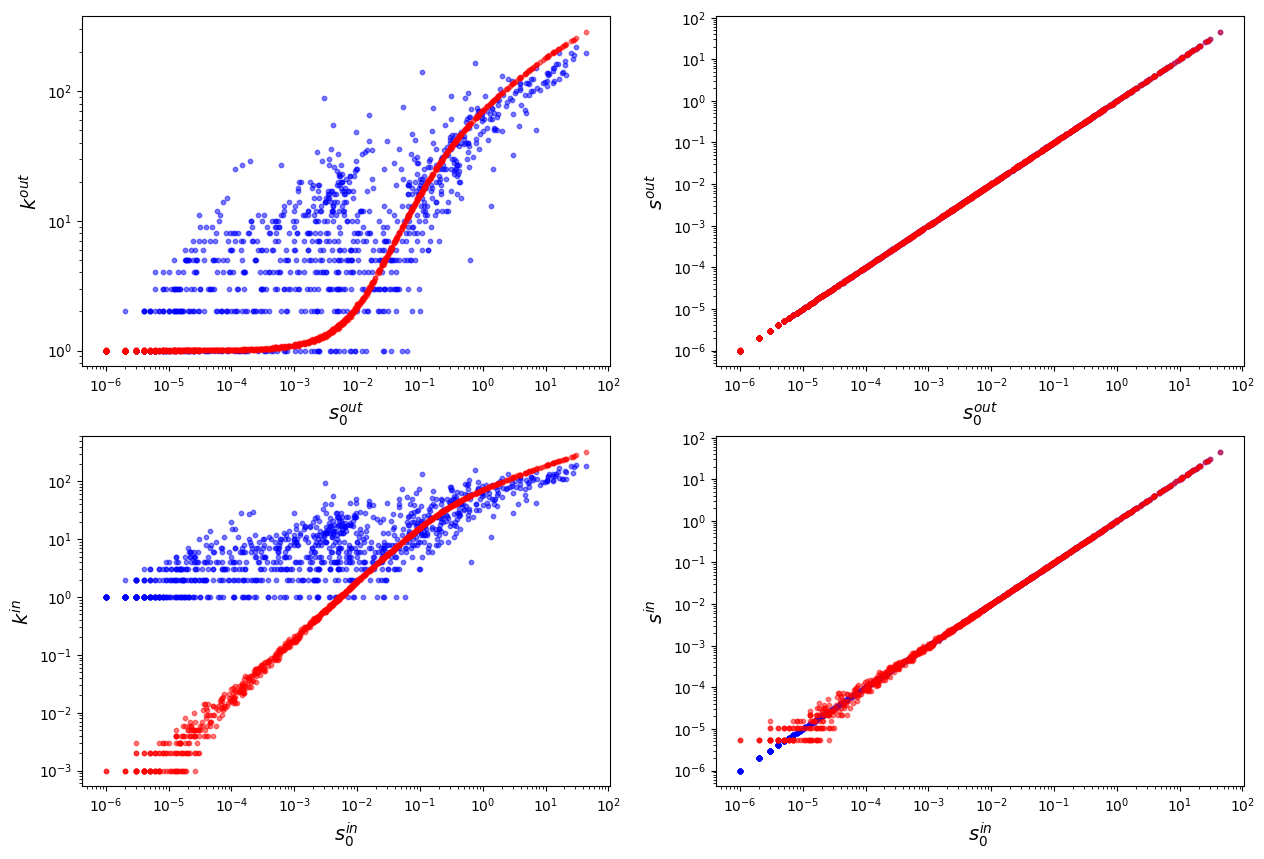
\includegraphics[scale=0.5]{../img/corrected_naive/degrees_strengths_rec.png}
    \caption{Comparison of both out-degrees, out-strengths and in-degrees, in-strengths. Blue points are nodes in the original ensemble, red points are averages of degrees or strengths over the ensemble for each node. Properties are compared against the $s_0^{out}$, the empirical out-strengths (strengths from the empirical ensemble).}
    \label{fig:degrees_strengths_rec_corrected_naive}
\end{figure}

In table \ref*{table:comparison_1}, we can see other results. Since we fitted $z$ specifically for the corrected model, we can see that the number of edges is again close to the one of the empirical graph. The number of out-isolated nodes is finally 0, on the other hand, the average number of in-isolated nodes even slightly increased. Also, the average maximum degree is higher than in the original model and significantly higher than in the empirical graph.

\begin{table}
\centering
\begin{tabular}{ |p{3cm}||p{2cm}|p{2cm}|p{2cm}|p{2cm}|  }
 \hline
 \multicolumn{4}{|c|}{Properties} \\
 \hline
 Property & Empirical network & SIM & Naive approach & Out-degree corrected SIM \\
 \hline
 Number of out-isolated nodes   & 0    &502.745&   200.101 & 0\\
 Number of in-isolated nodes   & 0    &503.166&   502.384 & 508.548\\
 Number of edges&   19199  & 19198.329  &19759.582 & 19195.15\\
 Maximal degree & 408 & 576.953&  611.876 & 602.796\\
 \hline
\end{tabular}
\caption{Comparison of the empirical network, original Scale-invariant model and its naive and corrected modifications.}
\label{table:comparison_1}
\end{table}

We can see that the number of isolated nodes decreased significantly, but they still form a fraction, which is not negligible.

\subsection{Correction of out-degrees and in-degrees simultaneously - Degree corrected SIM}
In the previous approach, we used the fact that we can sample out-links of each node independently. That was possible because we demanded only out-degrees to be nonzero. If we demand out-degrees and in-degrees to be nonzero simultaneously, we obtain dependence through the whole set of links, and we need to sample the whole graph at once.

The conditional probability of the whole graph configuration (which we denote $\{a_{ij}\}_{i,j=1}^N$) looks as follows

\begin{equation}
    P\left(\{a_{ij}\}_{i,j=1}^N \, | \, (k_i^{out} > 0 \, \forall i) \cap (k_i^{in} > 0 \, \forall i )\right) = \frac{P\left(\{a_{ij}\}_{i,j=1}^N \cap (k_i^{out} > 0 \forall i) \cap (k_i^{in} > 0 \forall i )\right)}{P\left((k_i^{out} > 0 \, \forall i) \cap (k_i^{in} > 0 \, \forall i )\right)}
\end{equation}

A configuration, which does not satisfy the conditions has zero probability. Let us denote the space of all possible graphs with $(k_i^{out} > 0 \, \forall i) \cap (k_i^{in} > 0 \, \forall i )$ as $\Gamma$. Then on this space, we can define a new random graph model given by graph probability $P_\Gamma$:
\begin{equation}
    P_\Gamma\left(\{a_{ij}\}_{i,j=1}^N\right) = \frac{P\left(\{a_{ij}\}_{i,j=1}^N\right)}{P\left((k_i^{out} > 0 \, \forall i) \cap (k_i^{in} > 0 \, \forall i )\right)} \qquad \forall \{a_{ij}\}_{i,j=1}^N \in \Gamma
\end{equation}
where $P$ is the probability induced by the original Scale-invariant model. 

The denominator (normalization constant, partition function) is difficult to compute. Also, if we could obtain probabilities for all configurations $\{a_{ij}\}_{i,j=1}^N$, it would still be usually hard to sample directly from the distribution obtained. We would have to sample the whole graph at once, and if the number of allowed configurations is high, each probability can be very low, and we could encounter numerical problems.

To avoid these obstacles, we propose to use the Metropolis-Hastings algorithm. The main advantage of it is that we do not to know the normalization function (partition sum) explicitly, as it only uses the ratio of probabilities.

We will proceed in the following manner:

\begin{enumerate}
\item We start from any configuration complying to our conditions. For example, we can connect node 1 to 2, 2 to 3 and so on to form a circle. Then we can add additional edges to have a similar number of edges as in the empirical graph.
\item We propose a new configuration by flipping any entry $a_{ij}$ of the adjacency matrix from 1 to 0 or from 0 to 1. We choose such entry uniformly randomly.
\item If the proposal does not comply to our condition, we refuse it and randomly choose entry $a_{ij}$ again. We do that until we obtain an allowed configuration.
\item Having an allowed proposal, we calculate the acceptance ratio. Since we flipped only entry $a_{ij}$, the ratio of probabilities of the proposal vs. the initial graph is $\alpha = \frac{p_{ij}}{1-p_{ij}}$ if the proposed $a_{ij} = 1$ or $\alpha = \frac{1-p_{ij}}{p_{ij}}$ if proposed $a_{ij} = 0$
\item We generate a uniform number $u \in [0,1]$. If $u\leq\alpha$, we accept the proposal, otherwise we keep the adjacency matrix from the previous step. Then we repeat the algorithm from step 2).
\end{enumerate}

The disadvantage of this approach is that we get highly autocorrelated series of graphs. Therefore, we can only choose each $i$-th graph from this procedure (this method is usually called thinning). The higher the $i$ is, the less autocorrelated ensemble we get. 

Also, it takes some time for the algorithm to reach the high-probability region, therefore we implement the so-called burn-in period, which means we discard the first $j$ samples.

\subsubsection{Finding a proper value of $z$}
This corrected model still depends on the value of $z$. We can not choose the same value of $z$ as in the original model, since we reject unplausible realizations of it and therefore our correction naturally increases the number of links compared to the original model. We need to fit $z$ according to the empirical network we have.

In this sense, we fit $z^*$ in such a way to replicate the number of links well. In the original SIM, we demanded
\begin{equation}
    L_0 = \langle L \rangle = \sum_{i,j} p_{ij} = \sum_{i,j} P(a_{ij} = 1) = \sum_{i,j} 1-\exp{(-z^*x_iy_j)}
\end{equation}
In the corrected model, things get more complicated. 
Let us first denote the marginal probability (denoted as $p_{ij}^M$) of every edge $a_{ij}$ as
\begin{equation}
    p_{ij}^M = \sum_{\{a_{kl}\} \in \Gamma, a_{ij} = 1} P_\Gamma\left(\{a_{ij}\}_{i,j=1}^N\right)
\end{equation}
i.e. we are summing probabilities of all possible configurations from $\Gamma$ where $a_{ij} = 1$. 

Then we get
\begin{align}
    \langle L \rangle &= \mathbb{E}_\Gamma\left(L\right) = \mathbb{E}_\Gamma\left(\sum_{i,j=1}^{N} a_{ij}\right) = \sum_{\{a_{kl}\} \in \Gamma} \sum_{i,j=1}^{N} a_{ij} P_\Gamma\left(\{a_{kl}\}\right) = \sum_{i,j=1}^{N} \sum_{\{a_{kl}\} \in \Gamma} a_{ij} P_\Gamma\left(\{a_{kl}\}\right)\\
    =&  \sum_{i,j=1}^{N} \sum_{\{a_{kl}\} \in \Gamma} a_{ij} P_\Gamma\left(\{a_{kl}\}\right) = \text{\{the case $a_{ij} = 0$ does not contribute\}} = \\
    =& \sum_{i,j=1}^{N} \sum_{\{a_{kl}\} \in \Gamma, a_{ij} = 1} P_\Gamma\left(\{a_{ij}\}_{i,j=1}^N\right) = \sum_{i,j=1}^{N} p_{ij}^M
\end{align}
which means, that instead of the probabilities from the original model, we should use marginal probabilities induced from our corrected model. However, the marginal probabilities are difficult to compute analytically. 

As an approximative workaround, we can find the value of $z^*$ by bisection on simulations. Since the number of links is on average increasing function of $z$, we can start with some guess, generate a corresponding ensemble, compute the average number of links, and if it's higher than the demanded number of links of the empirical network, we know we need to decrease $z$. Otherwise,x we increase it. Therefore, we can find value of $z^*$ using bisection to a demanded precision. The precision is not arbitrary, however, since there is a estimation error present, as we only estimate the number of links on the generated ensemble.

\subsubsection{Assigning weights}
The question remains, how to assign weights in this case. Our original model does it in the following way:
\begin{equation}
    w_{ij} = \frac{x_iy_j}{Wp_{ij}}
\end{equation}
where $p_{ij} = P(a_{ij} = 1)$. How do we replace $p_{ij}$?

Let us assume the weights are of form $w_{ij} = w(x_i, y_j)a_{ij}$. Then the expected out-strength of node $i$ in an ensemble is

\begin{align}
    \langle s_i^{out} \rangle &= \mathbb{E}_\Gamma\left(\sum_{j=1}^{N} w_{ij}\right) = \sum_{\{a_{kl}\} \in \Gamma} \sum_{j=1}^{N} w_{ij} P_\Gamma\left(\{a_{kl}\}\right) = \sum_{j=1}^{N} \sum_{\{a_{kl}\} \in \Gamma} w_{ij} P_\Gamma\left(\{a_{kl}\}\right) \\ &= \sum_{j=1}^{N} \sum_{\{a_{kl}\} \in \Gamma} w(x_i, y_j)a_{ij} P_\Gamma\left(\{a_{kl}\}\right) \\ &= \text{\{the case $a_{ij} = 0$ does not contribute\}} \notag \\
    &= \sum_{j=1}^{N} w(x_i, y_j) \sum_{\{a_{kl}\} \in \Gamma, a_{ij} = 1} P_\Gamma\left(\{a_{ij}\}_{i,j=1}^N\right) \\
    &= \sum_{j=1}^{N} w(x_i, y_j) p_{ij}^M
\end{align}

Therefore, we just need to assign $w(x_i, y_j) = \frac{x_i y_j}{W p_{ij}^M}$, because then
\begin{equation}
    \langle s_i^{out} \rangle = \sum_{j=1}^{N} w(x_i, y_j) p_{ij}^M = \sum_{j=1}^{N} \frac{x_i y_j}{W p_{ij}^M} p_{ij}^M = x_i \frac{\sum_{j=1}^{N} y_j}{W} = x_i
\end{equation}
which means we obtain the correct out-strength $x_i$ on average. This means we only need to obtain the marginal probabilities for each link to assign weights. As we know from estimation of $z$, we know it is hard to compute this probability analytically. However, we can estimate it as well. 

We generate an ensemble using our corrected model. This yields an ensemble of average matrices, from which we can compute an average adjacency matrix. Entries of this average adjacency matrix can be used as estimates of the marginal probabilities.

\subsubsection{Results}
We used the Metropolis-Hastings algorithm as explained above. The first configuration we use is the one where we connect node 1 to node 2, node 2 to node 3 etc. and then add uniformly randomly edges to obtain exactly $19\mathpunct{}199$ edges, same as in the empirical graph. Then, we had to find a corresponding value of $z$. Depending on how big samples we use for that, we can obtain a better estimate. Using bisection method, we obtained $z\approx 0.253$. Using this value, we can start sampling. We retained only each $1\mathpunct{}000\mathpunct{}000$-th sample (thinning). This ensures that each edge got a chance to flip approximately once before we take another sample (since we have 1021 vertices). This way, we generated $20\mathpunct{}000$ samples.

Let us first plot, how the number of edges changes during the sampling. That can be seen on figure \ref*{fig:num_links_MH}. We can clearly observe that in the beginning of the sampling, the number of edges increases quickly. This is the period, when the sampling still searches for the most-probable configurations. T avoid undesirable biases, we discard first $10\mathpunct{}000$ samples and only keep the rest. Also, it seems that even in the later stage of sampling, the number of edges still keeps increasing slowly. That means that the maximally probable configurations still might not have been fully found and to improve the results, we might need to run the sampling even longer. 

\begin{figure}[!ht]
    \centering
    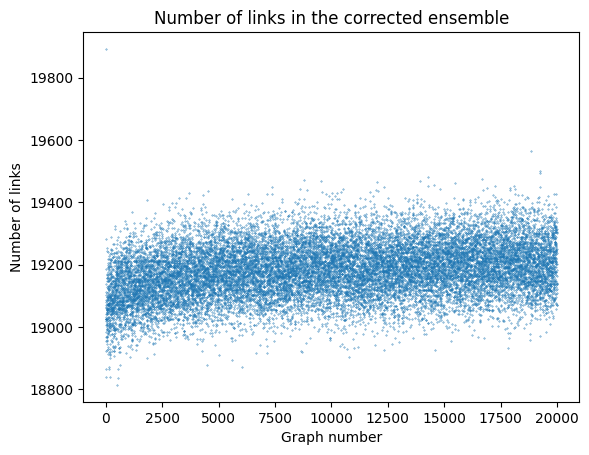
\includegraphics[scale=0.8]{../img/metropolis/num_links.png}
    \caption{Number of edges of each graph in the sampled ensemble, as the sampling went in time. We can see that in the beginning, the number of edges increases fast, therefore we should use a burn-in period.}
    \label{fig:num_links_MH}
\end{figure}

Secondly, to study if our sampling method reaches the highly probable states, we might take a closer look at some bias we might have introduced. The sample we start the algorithm with is a one where we connected nodes in a circle (node 1 to node 2 etc.) and we can thus study, how many of these edges stay retained after some period of sampling. We expect that the highly improbable edges vanish very quickly. If the number of retained edges reaches some steady state, we might say we reached some sort of equilibrium. 

The result can be seen on figure \ref*{fig:second_diagonal}. The number of preserved edges drops very quickly, but seems to be slightly decreasing even after $10\mathpunct{}000$-th sample. This also suggests, that to reach equilibrium, we would need much longer sampling. 

\begin{figure}[!ht]
    \centering
    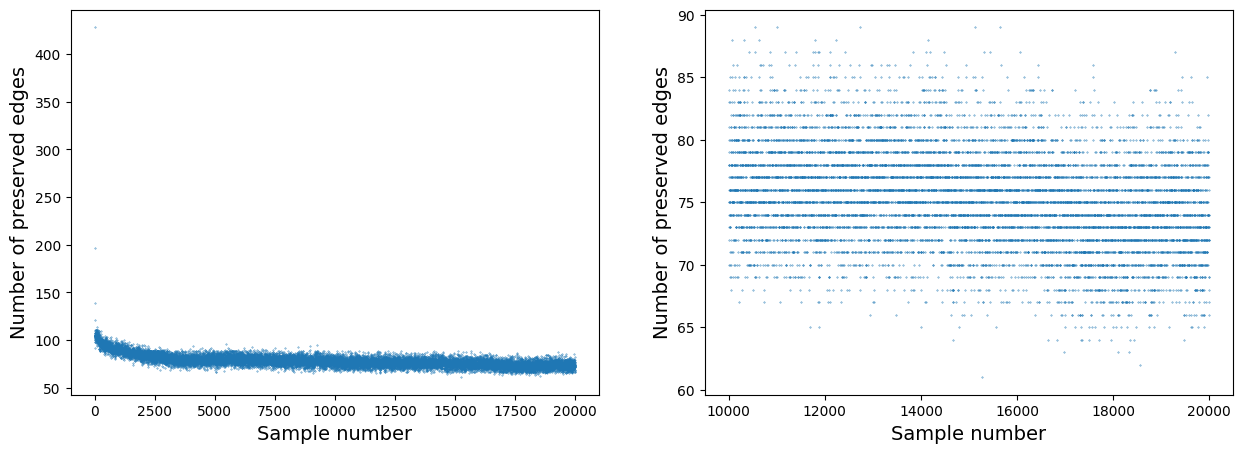
\includegraphics[scale=0.5]{../img/metropolis/second_diagonal.png}
    \caption{Number of edges on the ``second diagonal'' (i.e. $a_{12}, a_{23}, a_{34}$ and so on) which are retained during the sampling. Our initial sample connects edge 1 to 2, 2 to 3, ..., 1021 to 1, so initially there were 1021 such edges. After few samples, the number drops significantly and seem to decrease even after many samples. On the left we show the whole sampling procedure, on the right figure only after $10\mathpunct{}000$-th sample.}
    \label{fig:second_diagonal}
\end{figure}

Next, we are supposed to assign weights, for which we need the estimates of marginal probabilities for every edge. For that, we take samples from the $10\mathpunct{}000$-th on and compute the average adjacency matrix of these samples. Its entries are then the estimates of marginal probabilities. 

Similar to the original model, we can study if strengths were assigned well by comparing them with the empirical strengths. Figure \ref*{fig:degrees_strengths_corrected} shows that strengths are reproduced well for nodes with high empirical strengths, however, the nodes with lower empirical strengths have on average lower than demanded strength in the ensemble. Let us recall, that in case of Out-degree corrected SIM, we got perfect reconstruction (figure \ref*{fig:degrees_strengths_rec_corrected_naive}). There, we computed the marginal probabilities analytically, here, on the other hand, we had to use an estimate given by the average adjacency matrix. This can lead in underestimation of strengths in the region of low empirical strengths. 

The graphs to the left on the figure \ref*{fig:degrees_strengths_corrected} show the comparison of degrees. Here we see that indeed, both in- and out-degrees are corrected and reproduced better, unlike in the situation, where we only corrected out-degrees (figure \ref*{fig:degrees_strengths_rec_corrected_naive})
\begin{figure}[!ht]
    \centering
    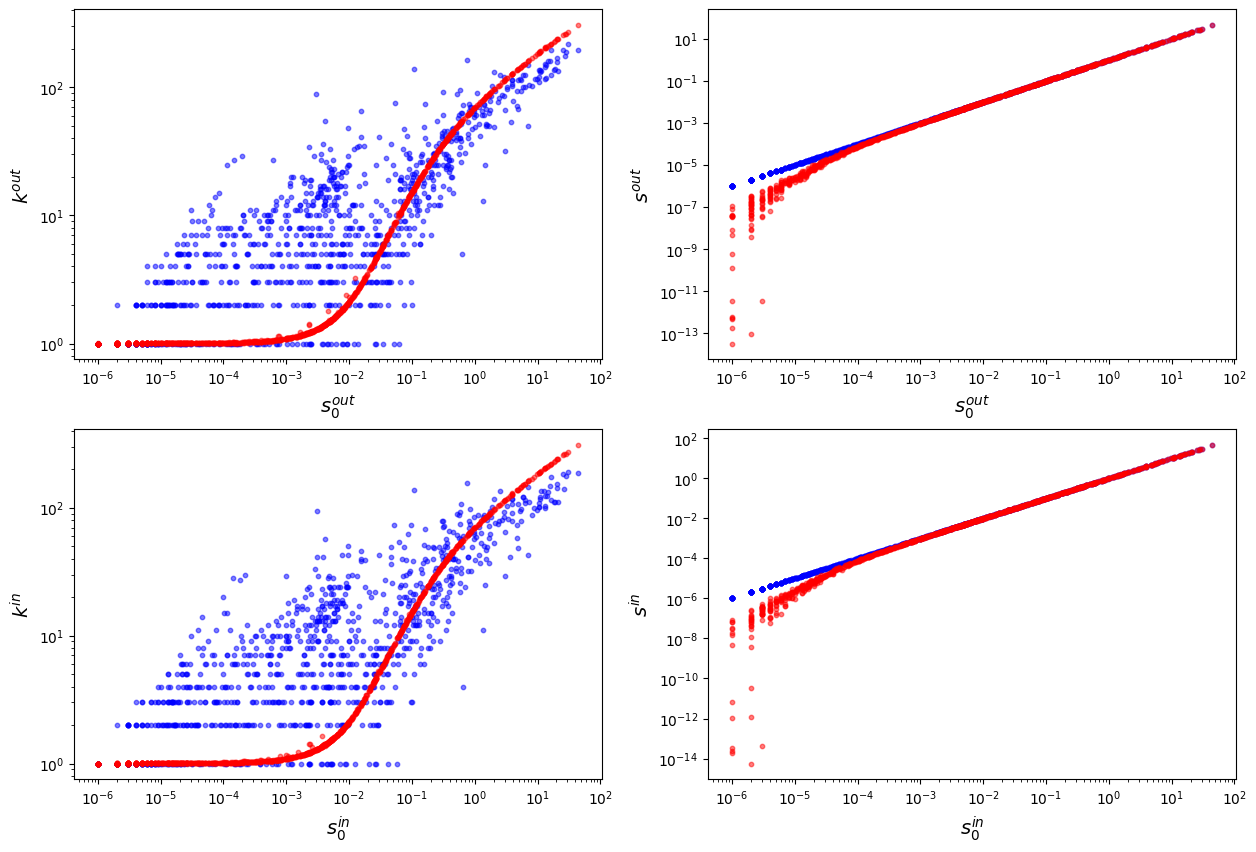
\includegraphics[scale=0.5]{../img/corrected/degrees_strengths_rec.png}
    \caption{Comparison similar to one on figures \ref{fig:deg_strengths_rec} and \ref*{fig:degrees_strengths_rec_corrected_naive}, but this time for the Degree corrected SIM.}
    \label{fig:degrees_strengths_corrected}
\end{figure}

Similarly to the original SIM, we may compare the histograms of degrees and strengths. Figure \ref*{fig:degrees_strengths_hist_corrected} shows for the degrees very similar results to those of the original SIM, apart from the case $k=1$. On the other hand, the results for strengths are very much different. Our degree-corrected model started producing nodes with much smaller strengths than which were observed in the empirical graph. Further investigation would be needed to show, whether it is due to limited size of the ensemble or it is a property of the model.

\begin{figure}[!ht]
    \centering
    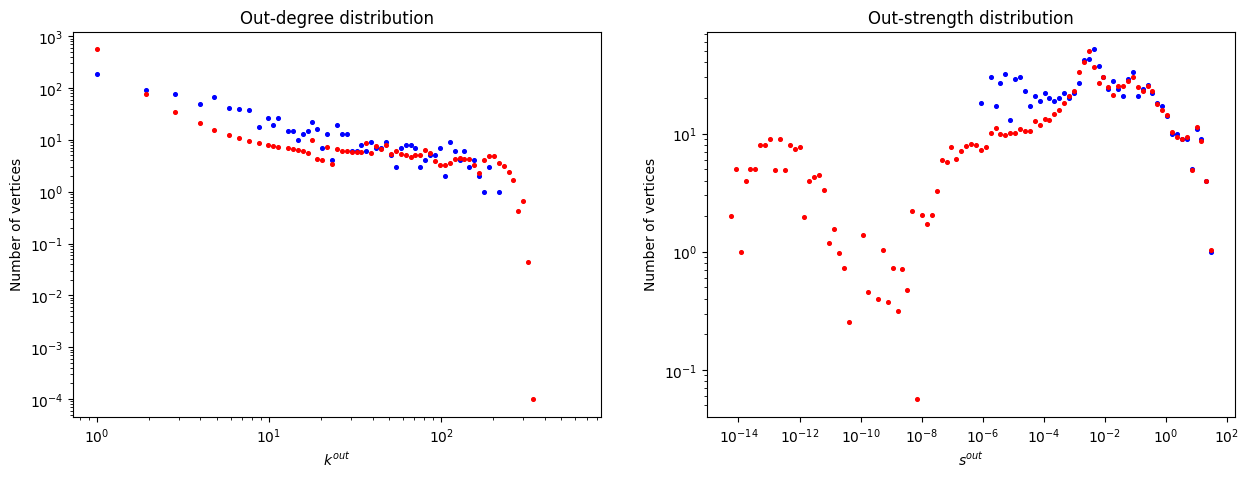
\includegraphics[scale=0.5]{../img/corrected/degrees_strengths_hist.png}
    \caption{Comparison of degree and strength histograms of the empirical graph and degree-corrected ensemble. }
    \label{fig:degrees_strengths_hist_corrected}
\end{figure}

We shall study the second order properties as well. First, let us focus on the ANND and ANNS (figure \ref*{fig:ANND_ANNS_corrected}). Compared to the original SIM (\ref*{fig:ANND_ANNS}), most of the nodes seem to follow similar pattern as in the original model, however, some of them start to manifest lowered ANND and ANNS. We investigated such nodes and found out, that they usually still keep their neighbor from the circle initialization of our sampling. We see that the problem is the more pronounced, the lower the empirical-strengths are. That is because in the Metropolis Hastings algorithm, it takes very long time for these nodes to obtain any other than the edge from the initialization, since any such edge is highly improbable. This could be solved by either waiting long enough or finding a better way to initialize the network. This just shows that even though the Metropolis-Hastings algorithm yields samples from the demanded distribution in the limit, it might actually take very long to truly replicate the distribution by sampling.

\begin{figure}[!ht]
    \centering
    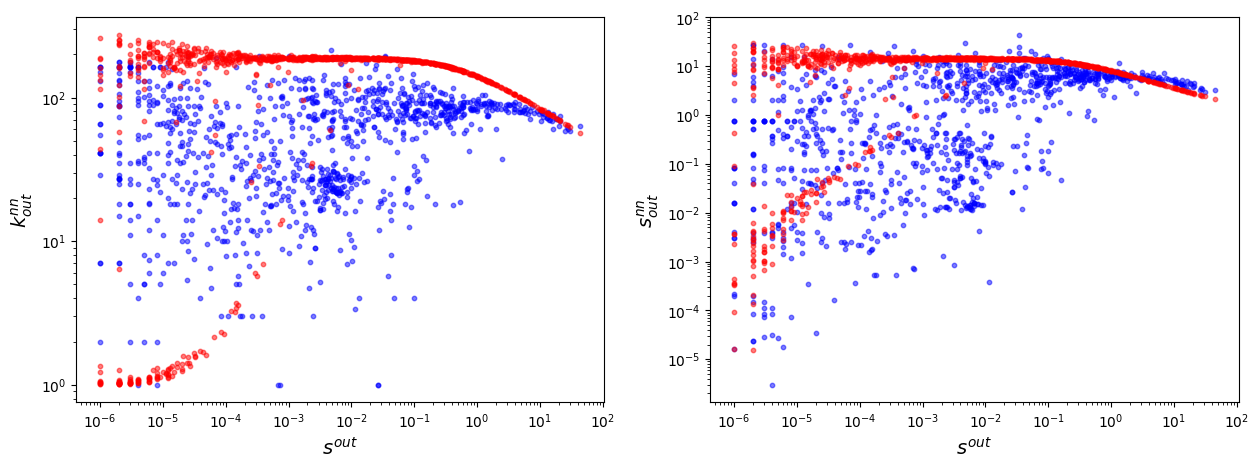
\includegraphics[scale=0.5]{../img/corrected/annd_anns.png}
    \caption{Comparison of ANND and ANNS for the original graph and its ensemble reconstruction using the Degree-corrected SIM. Compare with the original SIM (figure \ref*{fig:ANND_ANNS})}
    \label{fig:ANND_ANNS_corrected}
\end{figure}

Finally, we also show the aggregated version of ANND and local clustering coefficient for all nodes with the same degree (figure \ref*{fig:ANND_k_cl_coeff_k}, compare with figures \ref*{fig:ANND_k} and \ref*{fig:cl_coeff}). Compared with the original SIM, we notice only minor differences (with significant jump for $k=1$).

\begin{figure}[!ht]
    \centering
    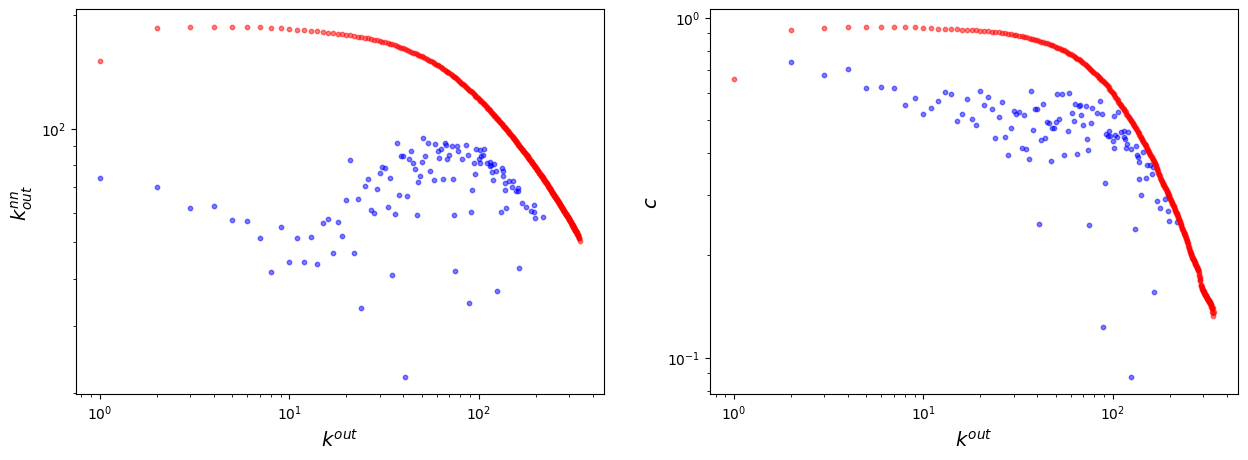
\includegraphics[scale=0.5]{../img/corrected/annd_k_cl_coeff_k.png}
    \caption{ANND and the local clustering coefficient, averaged for all nodes with the same degree (empirical network blue, ensemble reconstruction red). Compare with figures \ref*{fig:ANND_k} and \ref*{fig:cl_coeff}}
    \label{fig:ANND_k_cl_coeff_k}
\end{figure}

We might therefore conclude, that we obtained such a modification of the SIM, which achieved the nonzero degrees for each node while changing the other properties only in a very minor way. This is a good sign on one hand, on the other hand we might have hoped, that having the nonzero degrees would for example solve the problem of poor ANND reconstruction. We shall, however also remind ourselves, that we do not aim for a model applicable to all real-world networks, we only try to find models which are more or less suitable for specific domains. Even though some properties were not reproduced well enough for the airport network, it does not mean they would not be reproduced well for the financial network.
\chapter*{Conclusion} % SEM NESAHEJTE!
\addcontentsline{toc}{chapter}{Conclusion} % SEM NESAHEJTE!
\markboth{Conclusion}{Conclusion}
In this research project, we introduced basic network models as well as the Scale-invariant model, outlined the problem of network reconstruction with a focus on financial networks and then applied the Scale-invariant model in the reconstruction problem. We encountered a significant problem using the original Scale-invariant model, where the model would produce samples with half of nodes ending up isolated on average. Since this would largely influence study of dynamical processes on such reconstructed networks, we proposed o modification of the original model and a sampling strategy, which can avoid the production of isolated nodes. We studied other properties of the corrected model compared to the original version and found out, that although the problem of isolated nodes was solved, the quality of reconstruction did not largely improve when studying other network properties.

Although we came with some novel ideas, several aspects still need to be studied to fully explore the strength of the Scale-invariant model in the problem of network reconstruction. First, we shall note that not every model is useful in every situation. Our primary aim was to use the model in the area of financial networks, however, the datasets are difficult to obtain. We therefore used the airport network data, which, as we noted, might have different properties than the financial networks. The first important step would be to study the model on the true networks of interest and ideally even recognize the range of applicability.

Secondly, we made several hypotheses, for example that in some situations the predictions are not precise enough because of the limited number of samples in our ensembles or that the Metropolis-Hastings algorithm did not yet reach the equilibrium configurations of networks. These hypotheses need to be proved true or wrong, which would, however, need larger computational capacity. 

Another important step would be to not only study new network properties as we did, but also the properties of dynamical processes, like DebtRank. Only by that, we can prove the usefulness of our method, if we can for example predict the stress propagation on the network, whose structure we do not fully know and which we need to first reconstruct. 

Last but not least, we shall recall that there already exist several network reconstruction methods, and we should therefore compare their performance with our method. Our first motivation was, that the Scale-invariant model may work better in situations, where multiple scales are present, however, we did not evaluate that hypothesis yet. Also, there exist quantitative methods to compare the quality of reconstruction methods (as mentioned for example in \cite*{Squartini2018}), which shall be used to show the quality of our method. 

To conclude, in this project, we only started research in a topic, which opened many interesting questions to be further investigated. We can not conclude yet whether the proposed method brings significant improvements over already existing ones. On the other hand, we proposed an approach to avoid the creation of isolated nodes, which can be used not only in our method. 
%%%%%%%%%%%%%%%%%%%%%%%%%%%%%%%%%%%%%%%%%%%%%%%%%%%%%%%%%%%



%%%%%%%%%%%% SEZNAM POUŽITÝCH ZDROJŮ (LITERATURA) %%%%%%%%%%%%
\printbibliography[heading=bibintoc]


%%%%%%%%%%%% PŘÍLOHY PRÁCE %%%%%%%%%%%%
\newpage % SEM NESAHEJTE!
\appendix % SEM NESAHEJTE!

% \chapter*{Appendix}
\addcontentsline{toc}{chapter}{Appendix}
\renewcommand{\thesection}{\Alph{section}}

\pagestyle{fancy}
\fancyfoot{}
\fancyhead[RO,LE]{\thepage}
\fancyhead[RE]{Appendix}
\fancyhead[LO]{\nouppercase{\rightmark}}
TBD

\end{document} % SEM NESAHEJTE! Konec.
